\chapter{Lampiran Pengujian Experimental}
\label{lamp:B}

\section{Pengumuman untuk AIF182100 pada 21-27 April}
\label{sec:aif182100-21-27Apr}
\begin{figure}[H]
	\centering  
	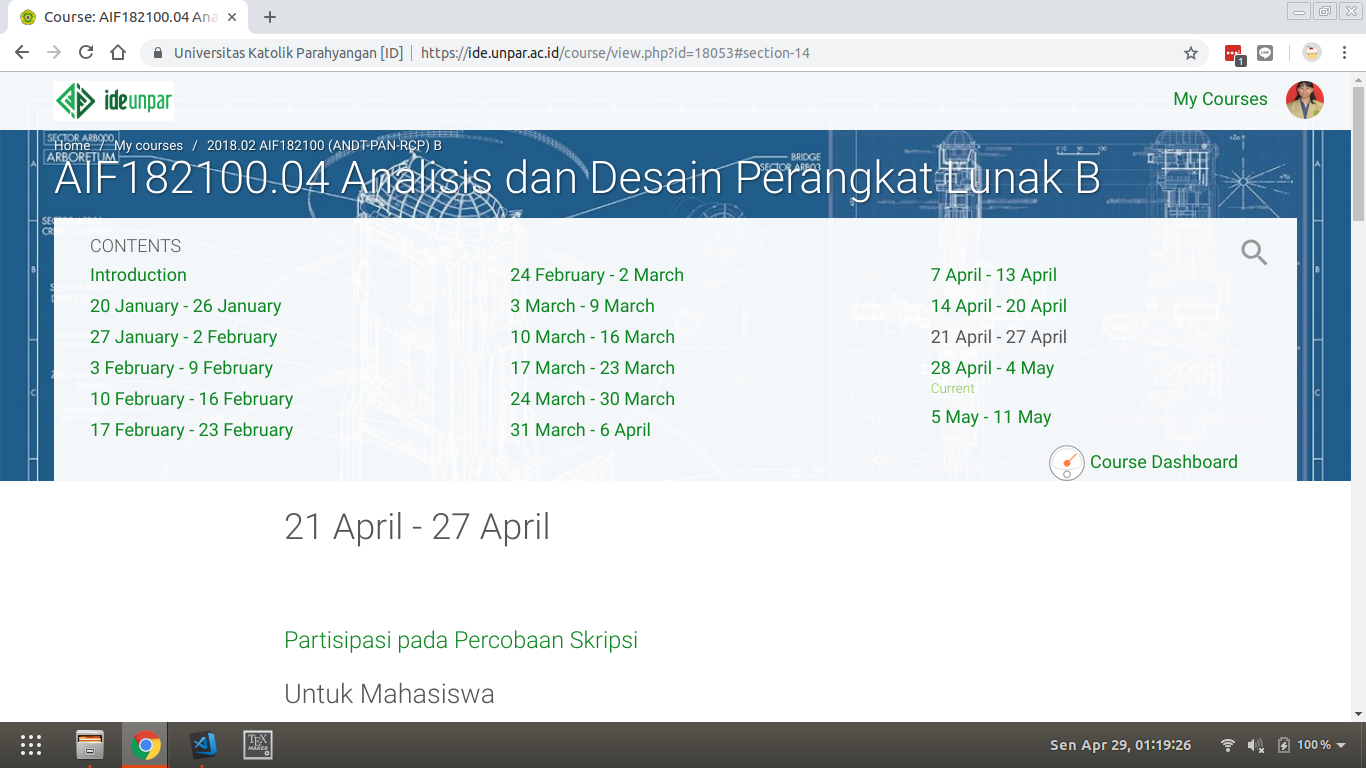
\includegraphics[width=\textwidth]{AIF182100-21-27April-Topbar.png}  
	\caption[Pengumuman di IDE UNPAR untuk AIF182100 pada 21-27 April]{Pengumuman di IDE UNPAR untuk AIF182100 pada 21-27 April} 
	\label{fig:AIF182100-21-27Apr} 
\end{figure}
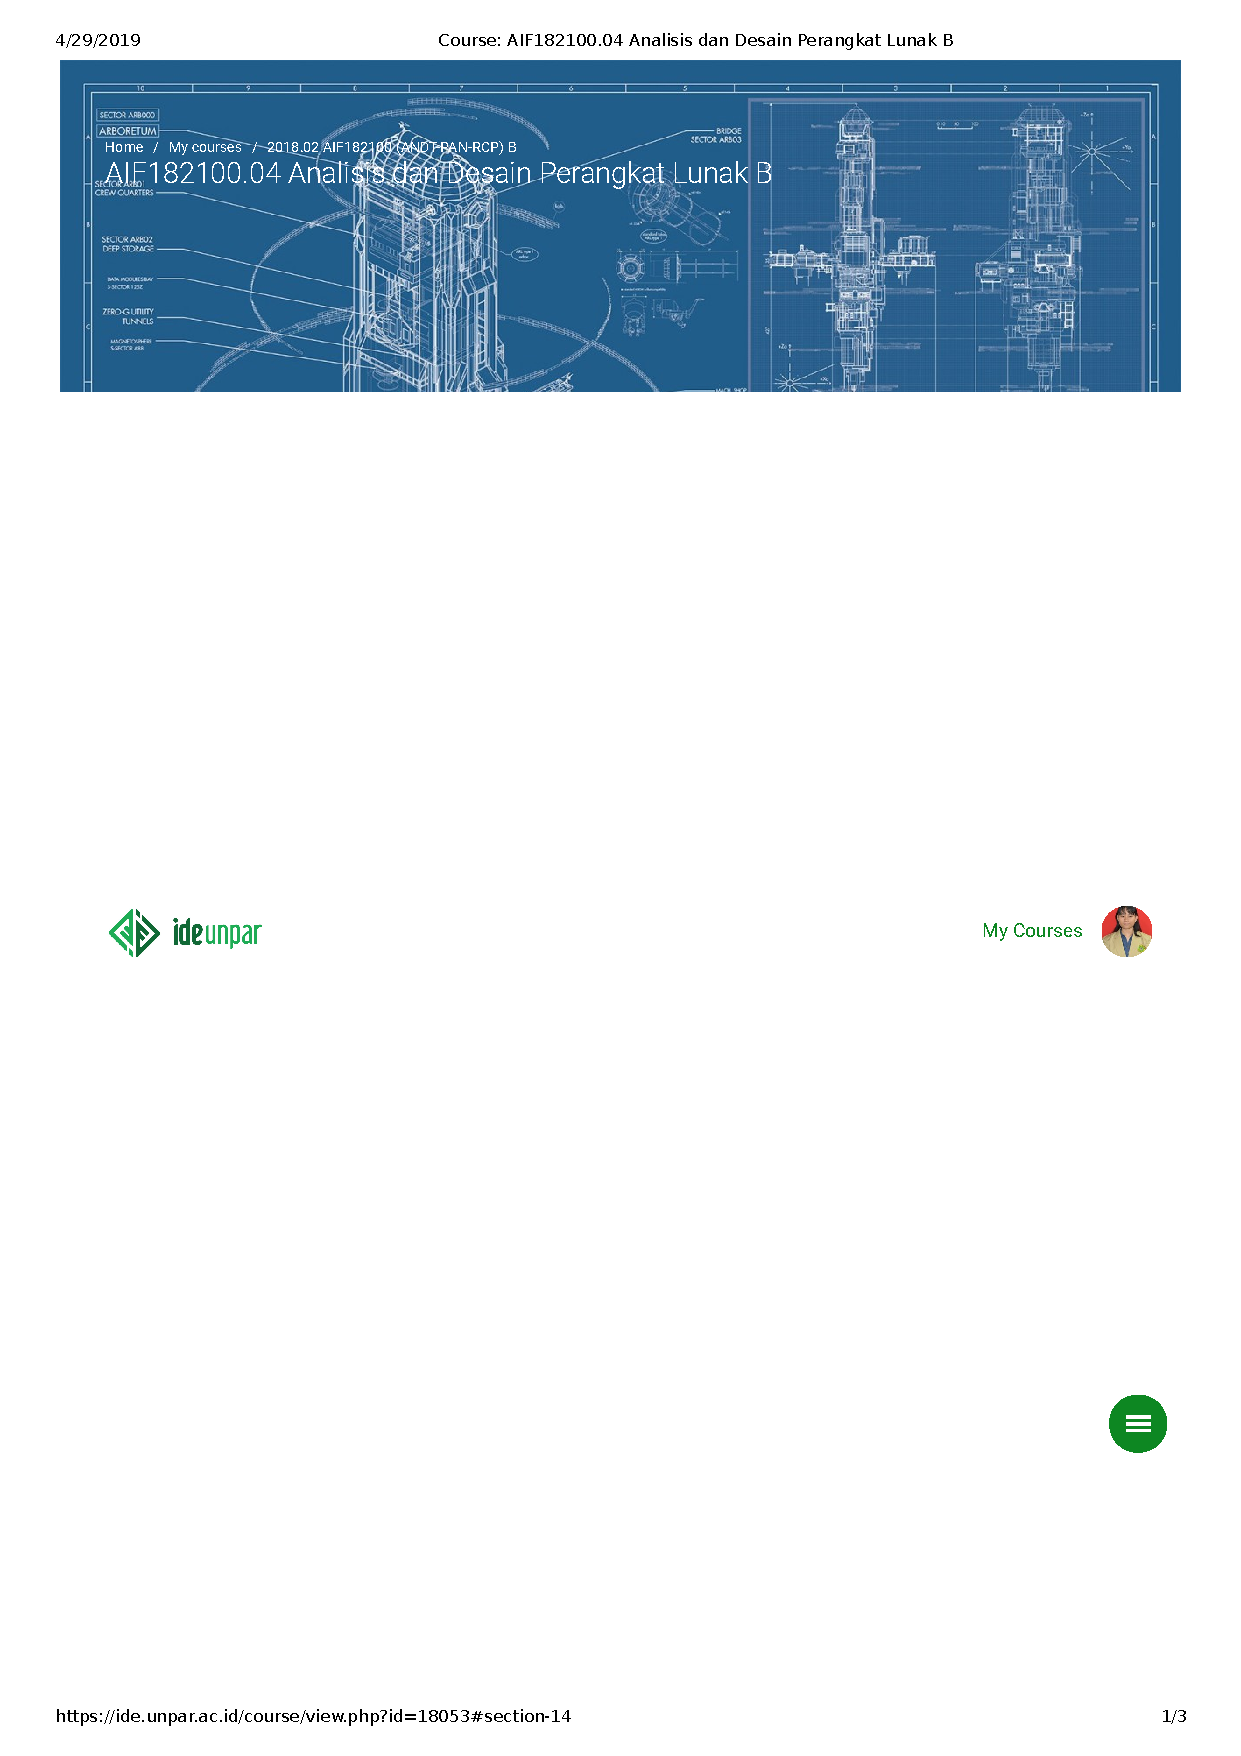
\includepdf[page=2-,pagecommand={},width=\textwidth]{./Lampiran/AIF182100-21-27April.pdf}

\section{Kuesioner}
\label{sec:survey}
Kuesioner diawali dengan pertanyaan :
\begin{figure}[H]
	\centering  
	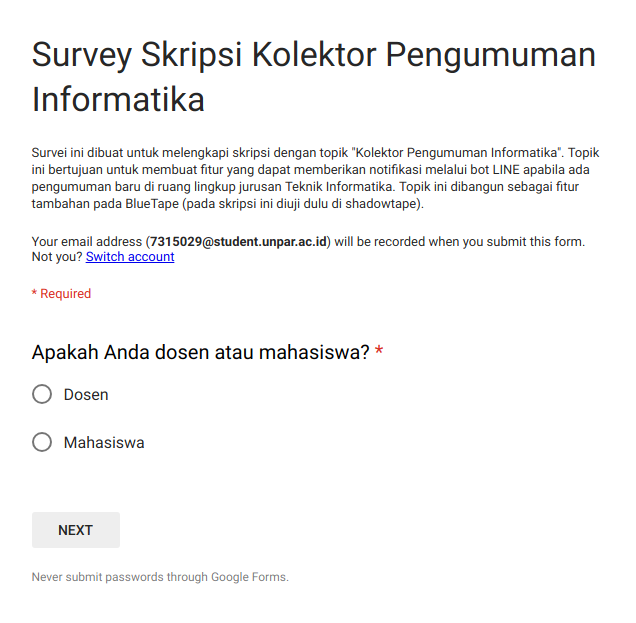
\includegraphics[scale=0.5]{./Survey-Kuesioner/Q0.png}  
	\caption[Kuesioner bagian pertama]{Kuesioner bagian pertama} 
	\label{fig:q0} 
\end{figure}

Apabila responden memilih "Dosen", maka responden akan dialihkan ke bagian Dosen (Lampiran \ref{subsec:survey-dosen}). Apabila responden memilih "Mahasiswa", maka responden akan dialihkan ke bagian Mahasiswa (Lampiran \ref{subsec:survey-mahasiswa}). Responden wajib mengisi semua pertanyaan di kuesioner ini kecuali pertanyaan saran.

\subsection{Dosen}
\label{subsec:survey-dosen}
\begin{figure}[H]
	\centering  
	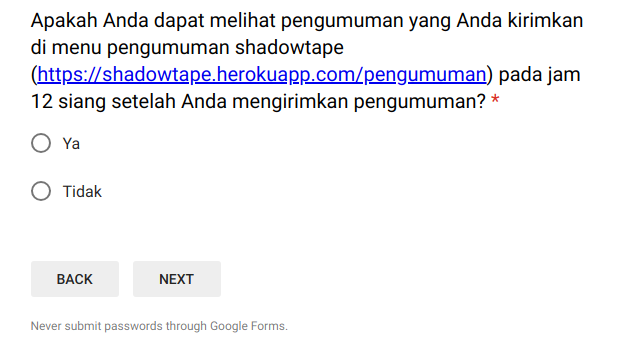
\includegraphics[scale=0.5]{./Survey-Kuesioner/Q1-D1.png}  
	\caption[Kuesioner bagian Dosen pertanyaan pertama]{Kuesioner bagian Dosen pertanyaan pertama} 
	\label{fig:q1-d1} 
\end{figure}

Apabila responden memilih jawaban "Ya" pada pertanyaan pertama (Gambar~\ref{fig:q1-d1}), maka responden akan dialihkan ke pertanyaan kedua (Gambar~\ref{fig:q1-d2}). Apabila responden memilih jawaban "Tidak", maka responden akan dialihkan ke bagian System Usability Scale dan Saran (Gambar~\ref{subsec:final}). 

\begin{figure}[H]
	\centering  
	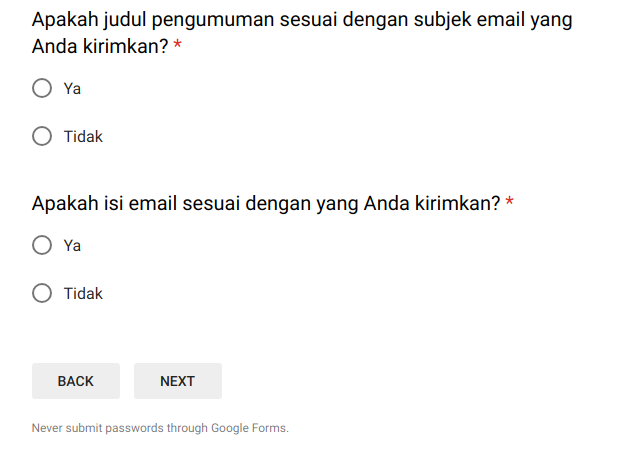
\includegraphics[scale=0.5]{./Survey-Kuesioner/Q1-D2.png}  
	\caption[Kuesioner bagian Dosen pertanyaan kedua dan ketiga]{Kuesioner bagian Dosen pertanyaan kedua dan ketiga} 
	\label{fig:q1-d2} 
\end{figure}

Apabila responden memilih jawaban "Ya" pada pertanyaan ketiga (pertanyaan kedua di Gambar~\ref{fig:q1-d1}), maka responden akan dialihkan ke pertanyaan keempat (Gambar~\ref{fig:q1-d3}). Apabila responden memilih jawaban "Tidak", maka responden akan dialihkan ke bagian System Usability Scale dan Saran (Gambar~\ref{subsec:final}). 

\begin{figure}[H]
	\centering  
	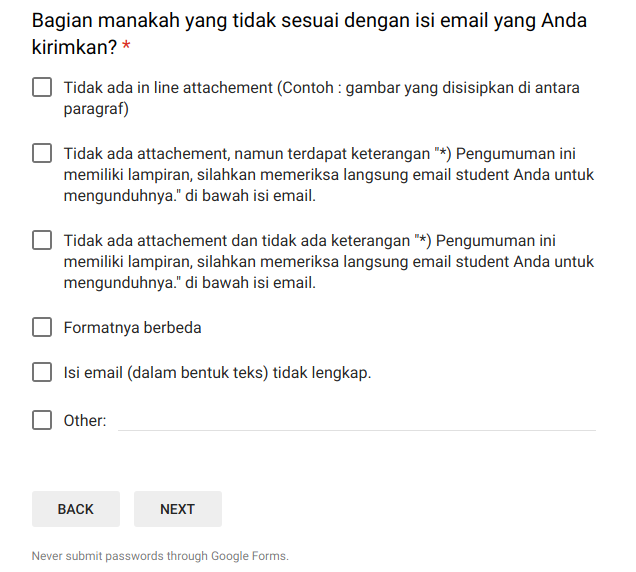
\includegraphics[scale=0.5]{./Survey-Kuesioner/Q1-D3.png}  
	\caption[Kuesioner bagian Dosen pertanyaan keempat]{Kuesioner bagian Dosen pertanyaan keempat} 
	\label{fig:q1-d3} 
\end{figure}

Apapun jawaban responden pada pertanyaan keempat (Gambar~\ref{fig:q1-d3}), responden akan dialihkan ke bagian System Usability Scale dan Saran (Gambar~\ref{subsec:final}).

\subsection{Mahasiswa}
\label{subsec:survey-mahasiswa}
\begin{figure}[H]
	\centering  
	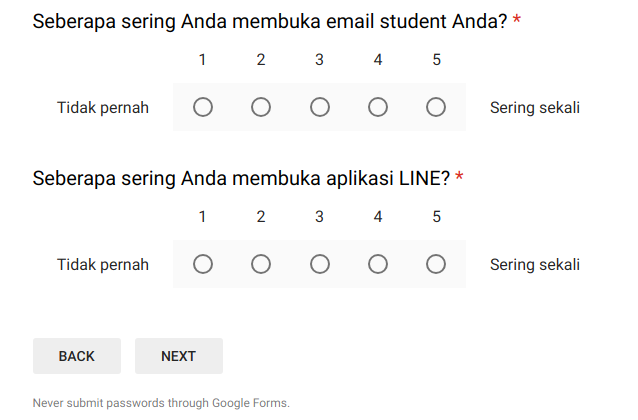
\includegraphics[scale=0.5]{./Survey-Kuesioner/Q1-M1.png}  
	\caption[Kuesioner bagian Mahasiswa pertanyaan pertama dan kedua]{Kuesioner bagian Mahasiswa pertanyaan pertama dan kedua} 
	\label{fig:q1-m1} 
\end{figure}

Apapun jawaban responden pada pertanyaan pertama dan kedua(Gambar~\ref{fig:q1-m1}), responden akan dialihkan ke pertanyaan kedua (Gambar~\ref{fig:q1-m2}).

\begin{figure}[H]
	\centering  
	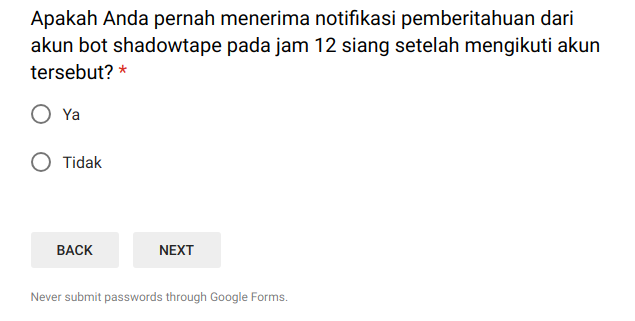
\includegraphics[scale=0.5]{./Survey-Kuesioner/Q1-M2.png}  
	\caption[Kuesioner bagian Mahasiswa pertanyaan ketiga]{Kuesioner bagian Mahasiswa pertanyaan ketiga} 
	\label{fig:q1-m2} 
\end{figure}

Apabila responden memilih jawaban "Ya" pada pertanyaan ketiga (Gambar~\ref{fig:q1-m2}), maka responden akan dialihkan ke pertanyaan keempat (Gambar~\ref{fig:q1-m3}). Apabila responden memilih jawaban "Tidak", maka jawaban responden akan dikirim kepada penulis.

\begin{figure}[H]
	\centering  
	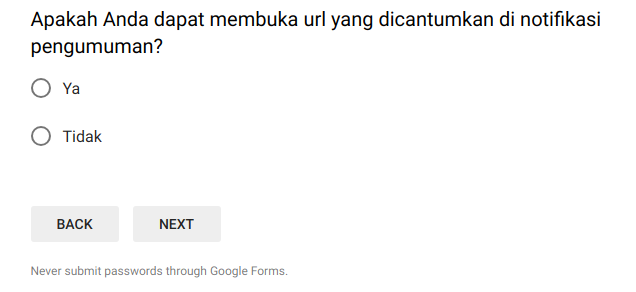
\includegraphics[scale=0.5]{./Survey-Kuesioner/Q1-M3.png}  
	\caption[Kuesioner bagian Mahasiswa pertanyaan keempat]{Kuesioner bagian Mahasiswa pertanyaan keempat} 
	\label{fig:q1-m3} 
\end{figure}

Apabila responden memilih jawaban "Ya" pada pertanyaan keempat (Gambar~\ref{fig:q1-m3}), maka responden akan dialihkan ke pertanyaan kelima (Gambar~\ref{fig:q1-m4}). Apabila responden memilih jawaban "Tidak", maka responden akan dialihkan ke bagian System Usability Scale dan Saran (Gambar~\ref{subsec:final}).

\begin{figure}[H]
	\centering  
	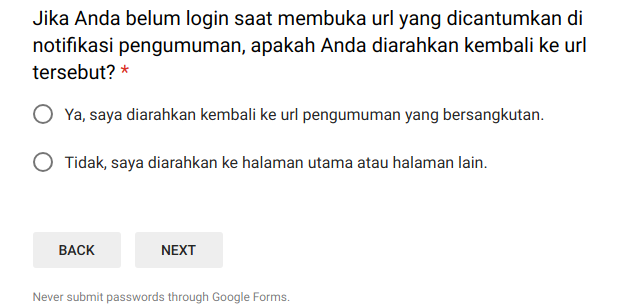
\includegraphics[scale=0.5]{./Survey-Kuesioner/Q1-M4.png}  
	\caption[Kuesioner bagian Mahasiswa pertanyaan kelima]{Kuesioner bagian Mahasiswa pertanyaan kelima} 
	\label{fig:q1-m4} 
\end{figure}

Apapun jawaban responden pada pertanyaan kelima (Gambar~\ref{fig:q1-m4}), responden akan dialihkan ke bagian System Usability Scale dan Saran (Gambar~\ref{subsec:final}).

\subsection{System Usability Scale dan Saran}
\label{subsec:final}

Bagian ini adalah bagian terakhir dari kuesioner. Setelah responden menjawab bagian ini, jawaban responden akan dikirim kepada penulis.

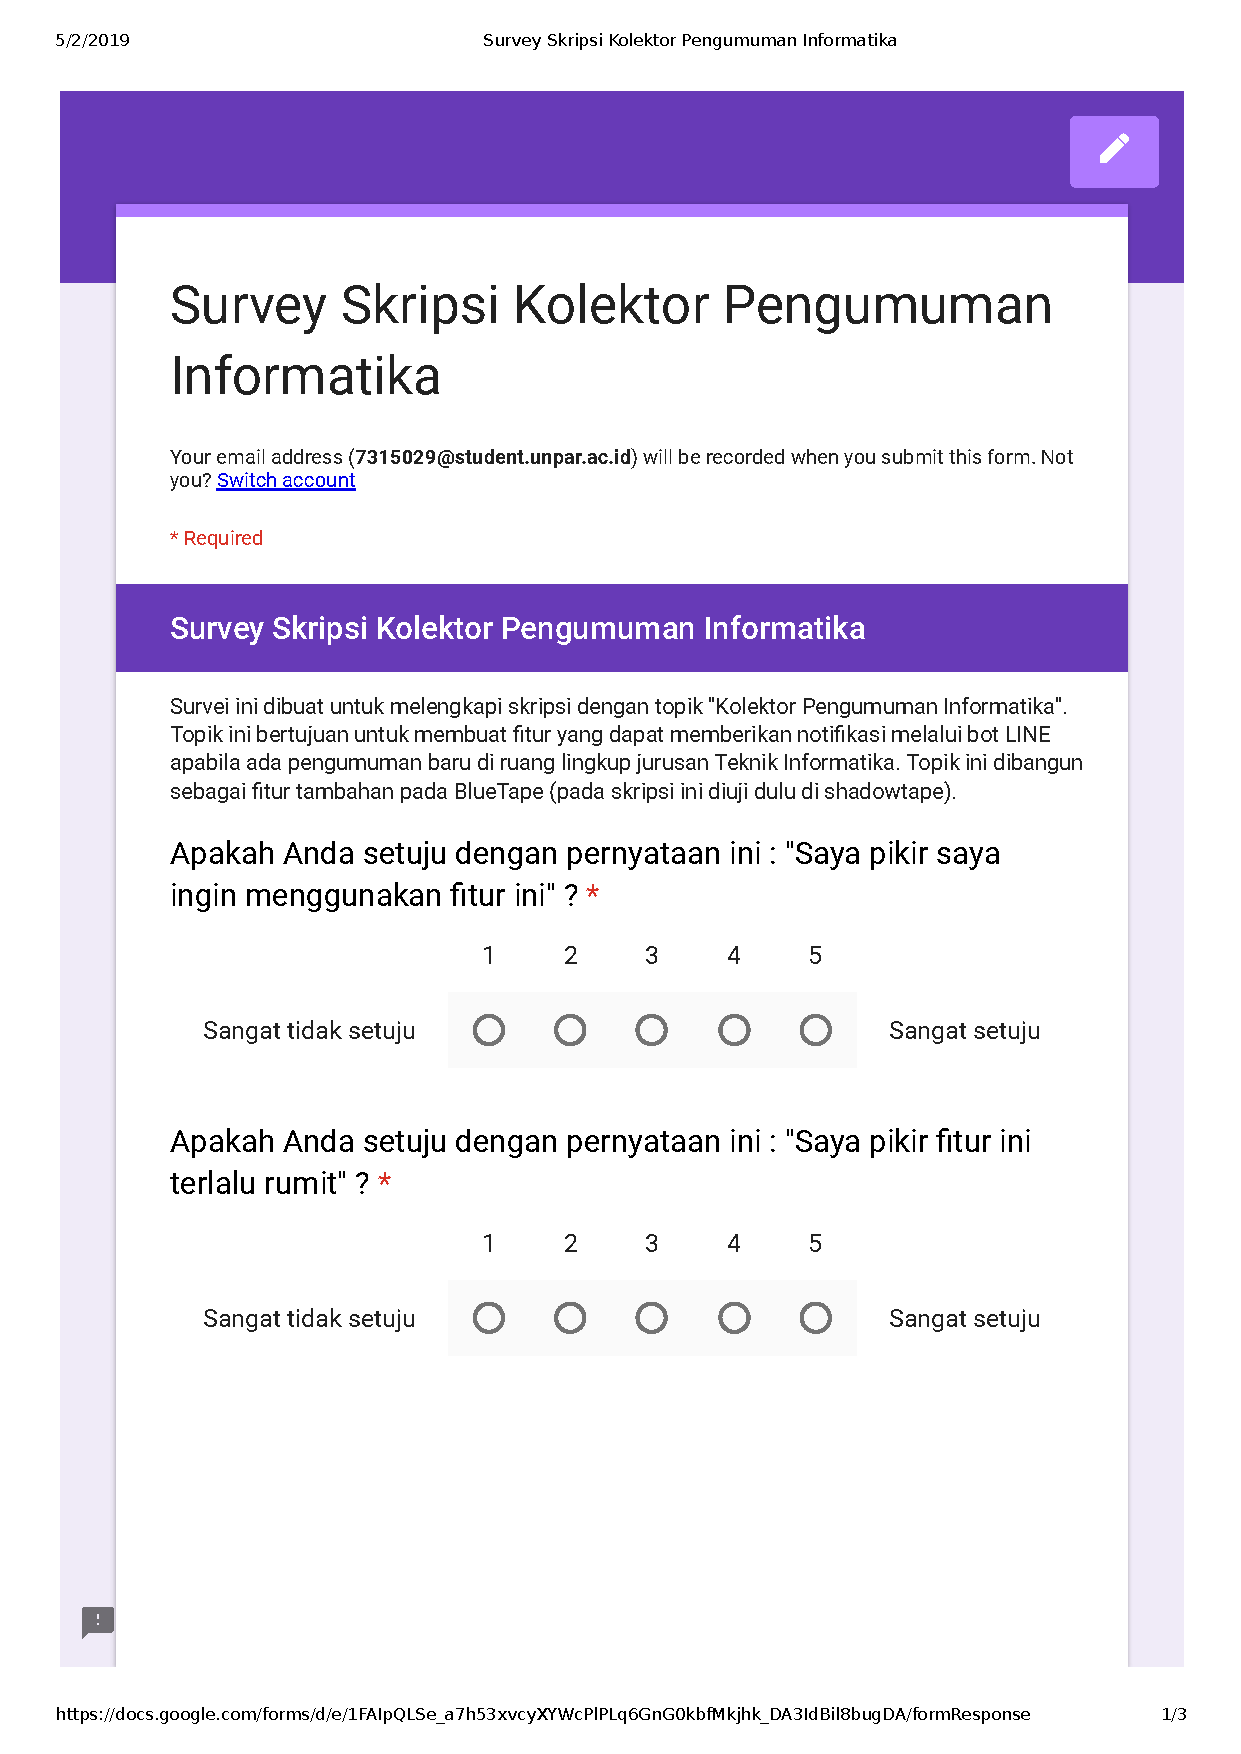
\includepdf[page=-,pagecommand={},width=\textwidth]{./Lampiran/Survey/Survey-LastQuestion.pdf}

\label{sec:full-result-survey}
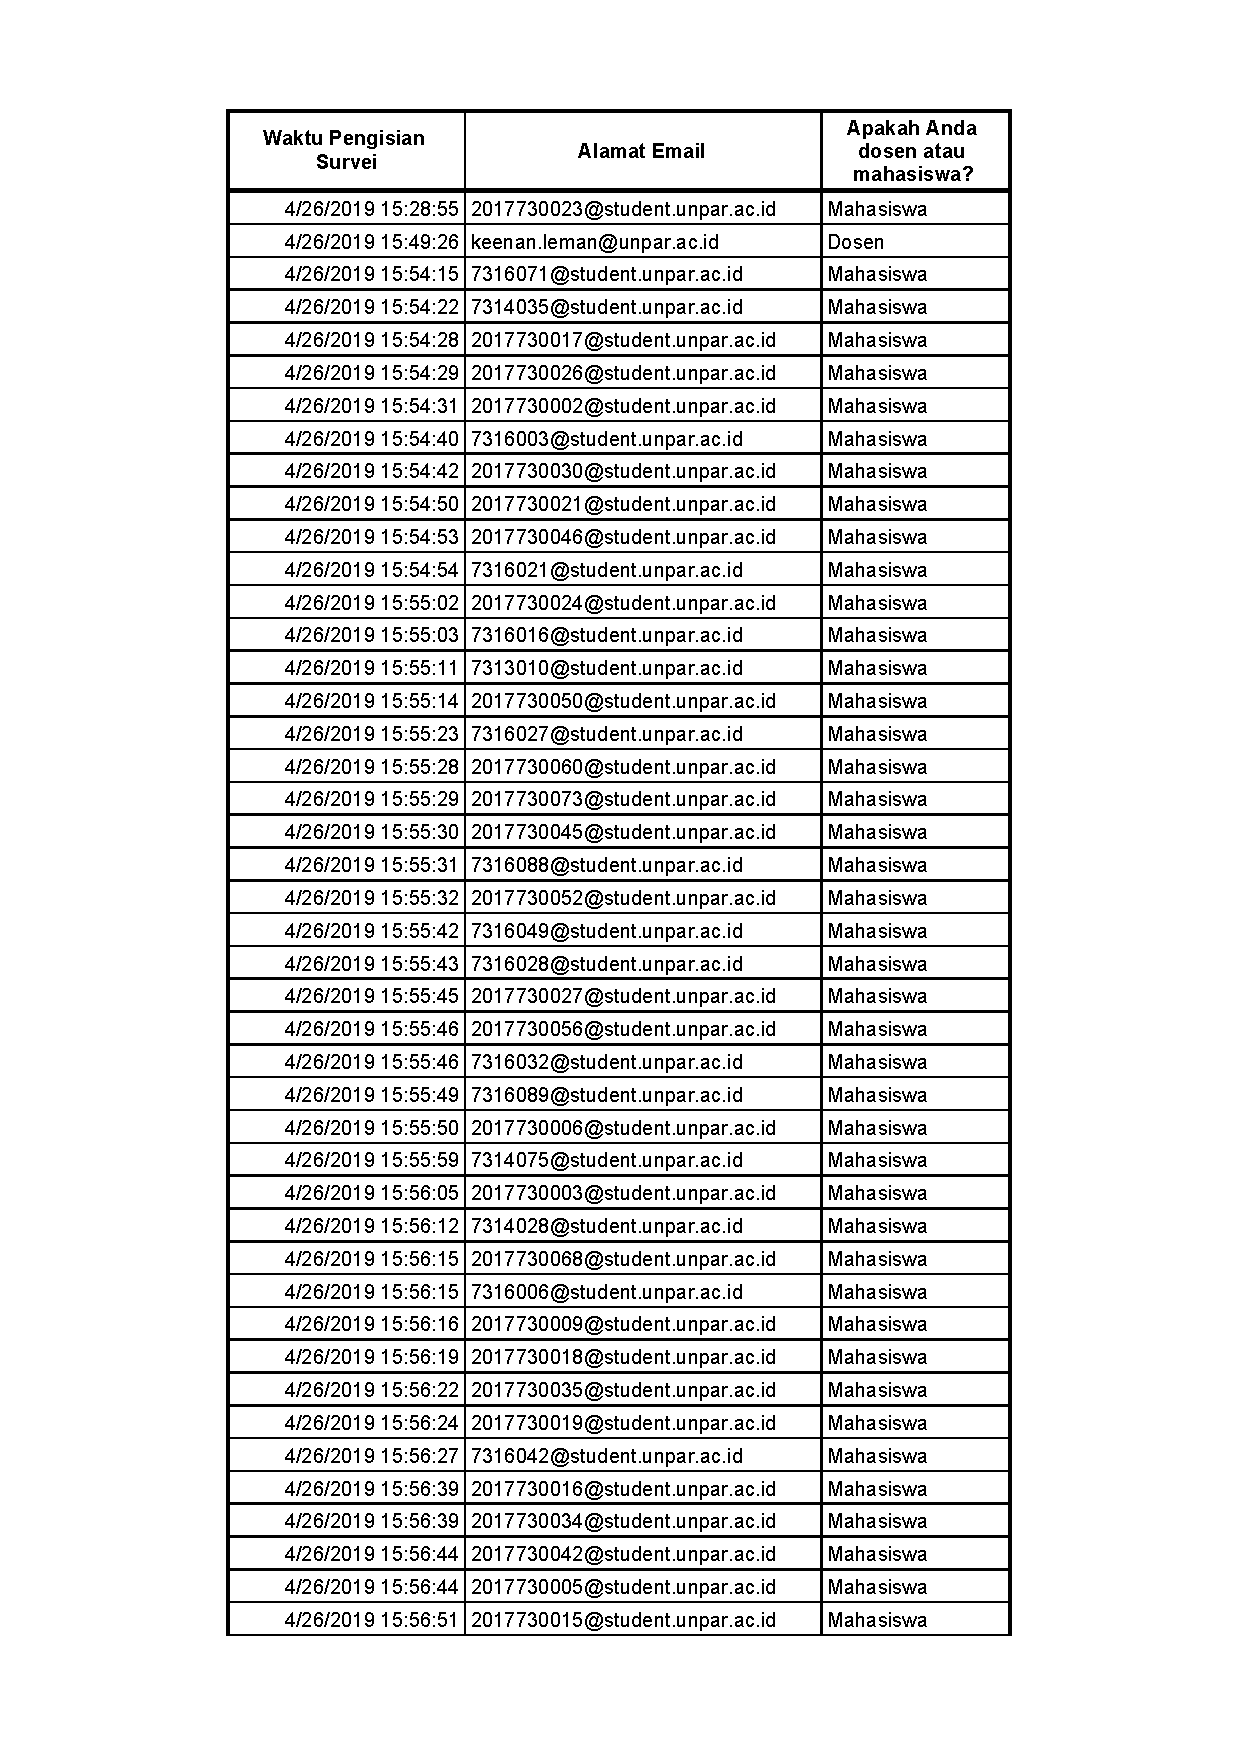
\includepdf[scale=0.8,page=1,pagecommand={\section{Hasil Mentah Kuesioner}}]{./Lampiran/Survey/Survey-DaftarPeserta.pdf}
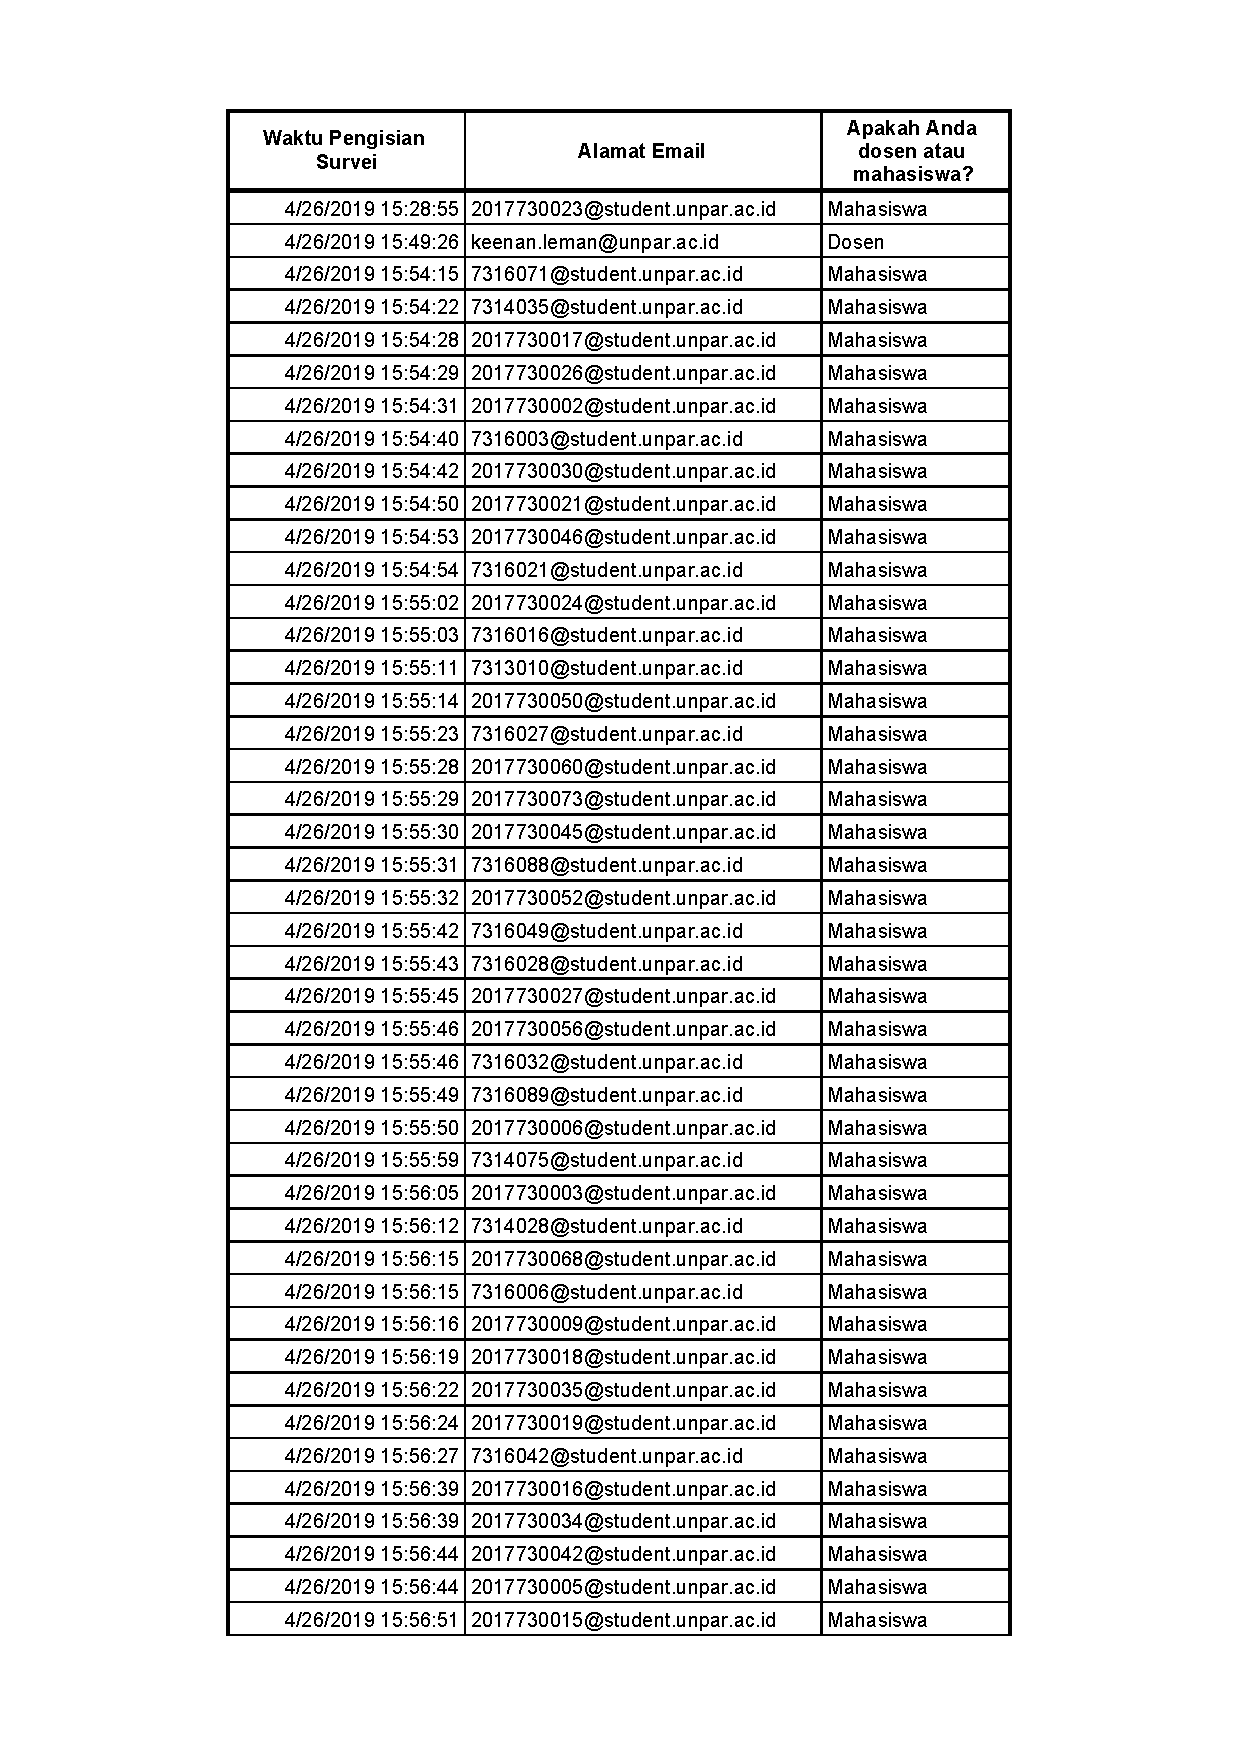
\includepdf[page=2-,pagecommand={},width=\textwidth]{./Lampiran/Survey/Survey-DaftarPeserta.pdf}
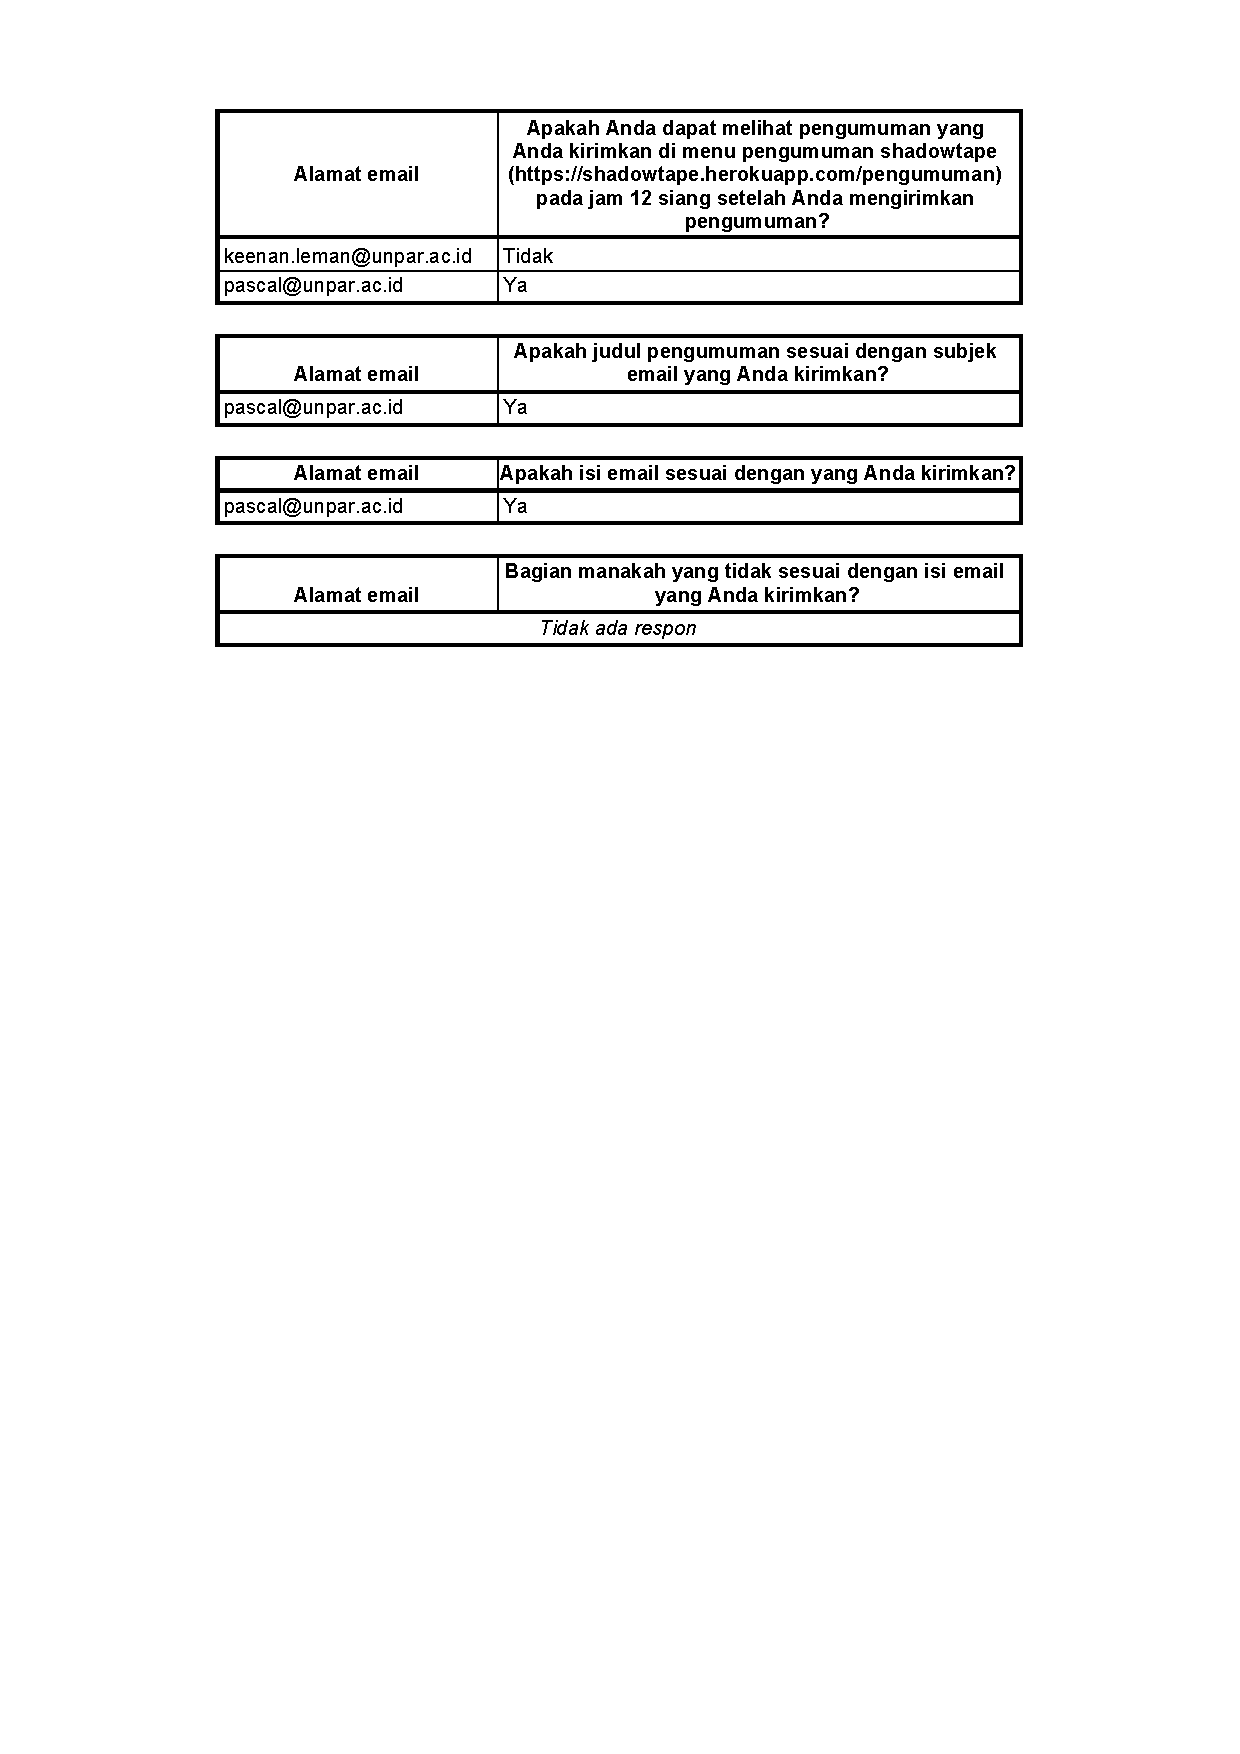
\includepdf[page=-,pagecommand={},width=\textwidth]{./Lampiran/Survey/Survey-Dosen.pdf}
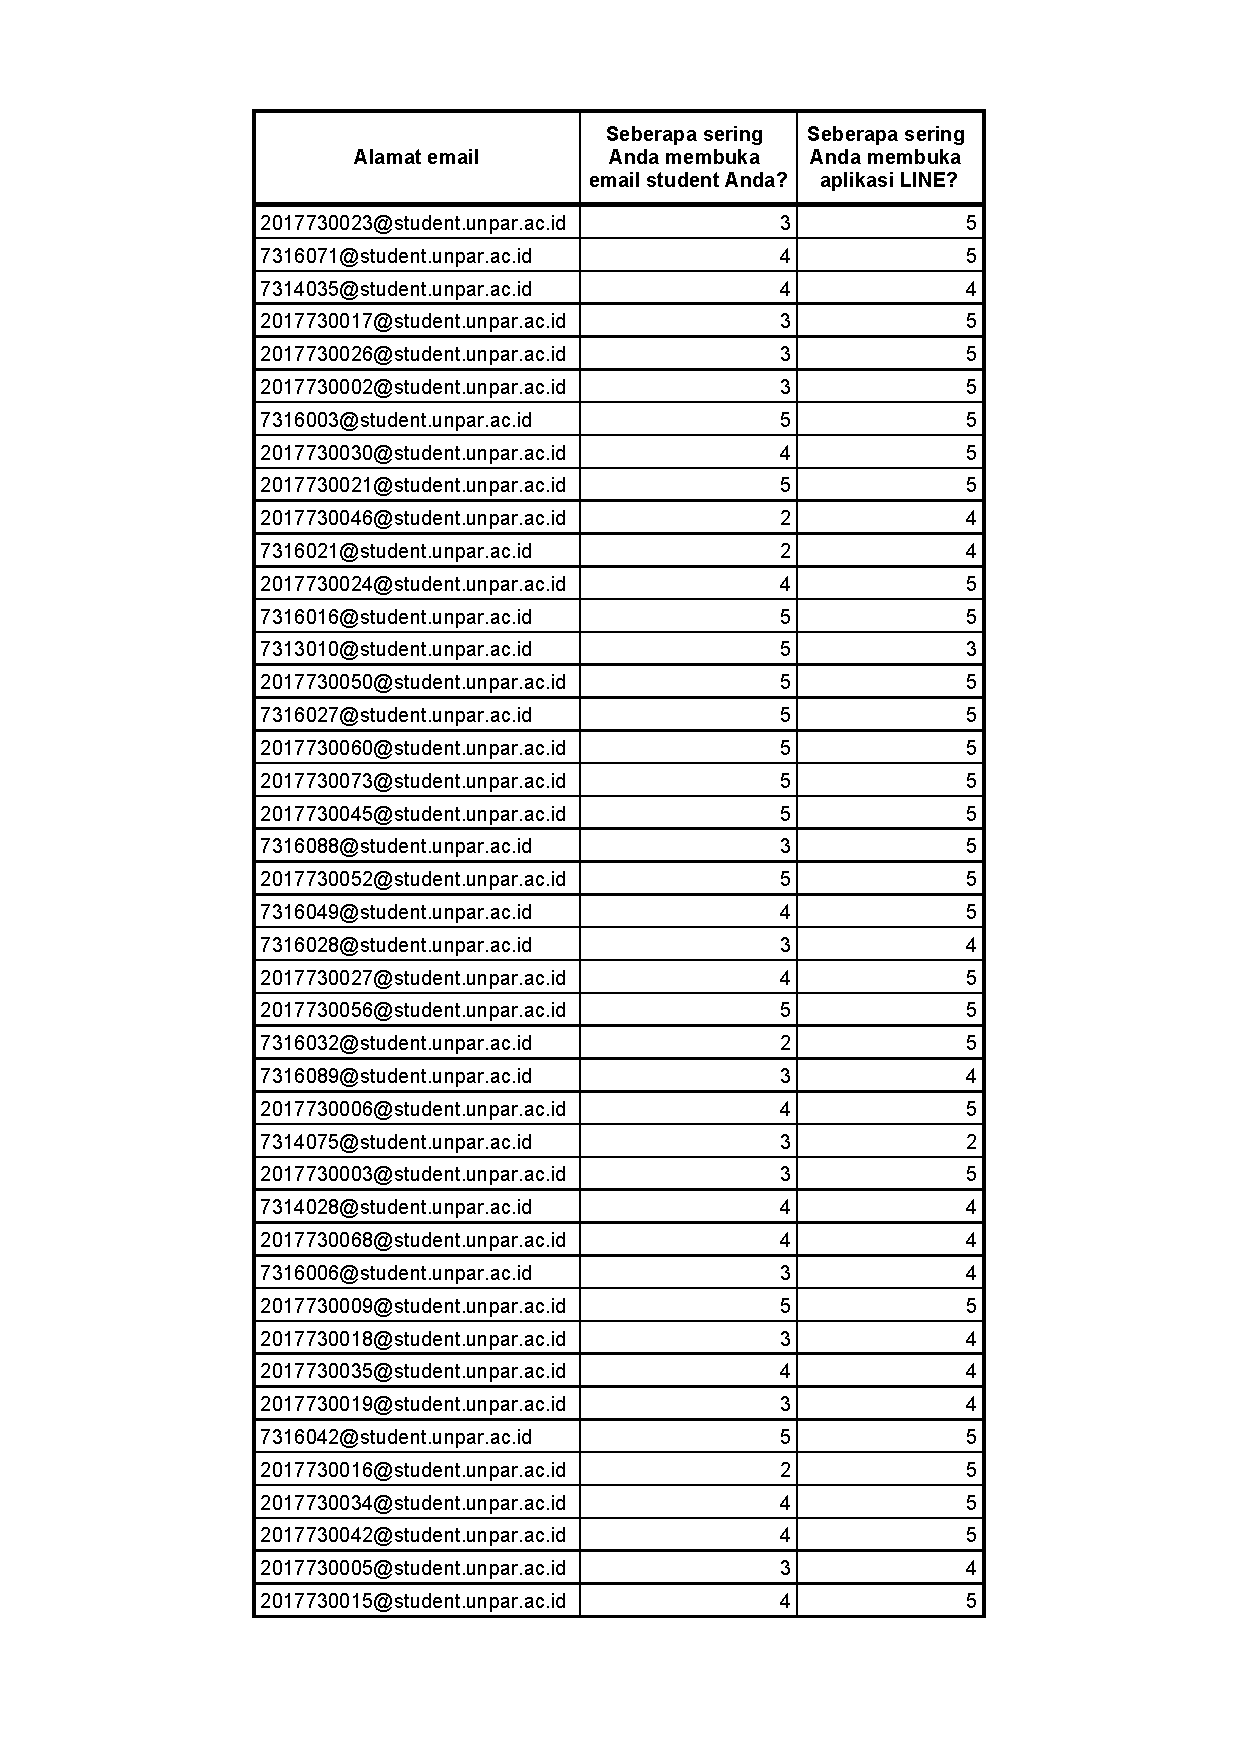
\includepdf[page=-,pagecommand={},width=\textwidth]{./Lampiran/Survey/Survey-PenggunaanEmaildanLINE.pdf}
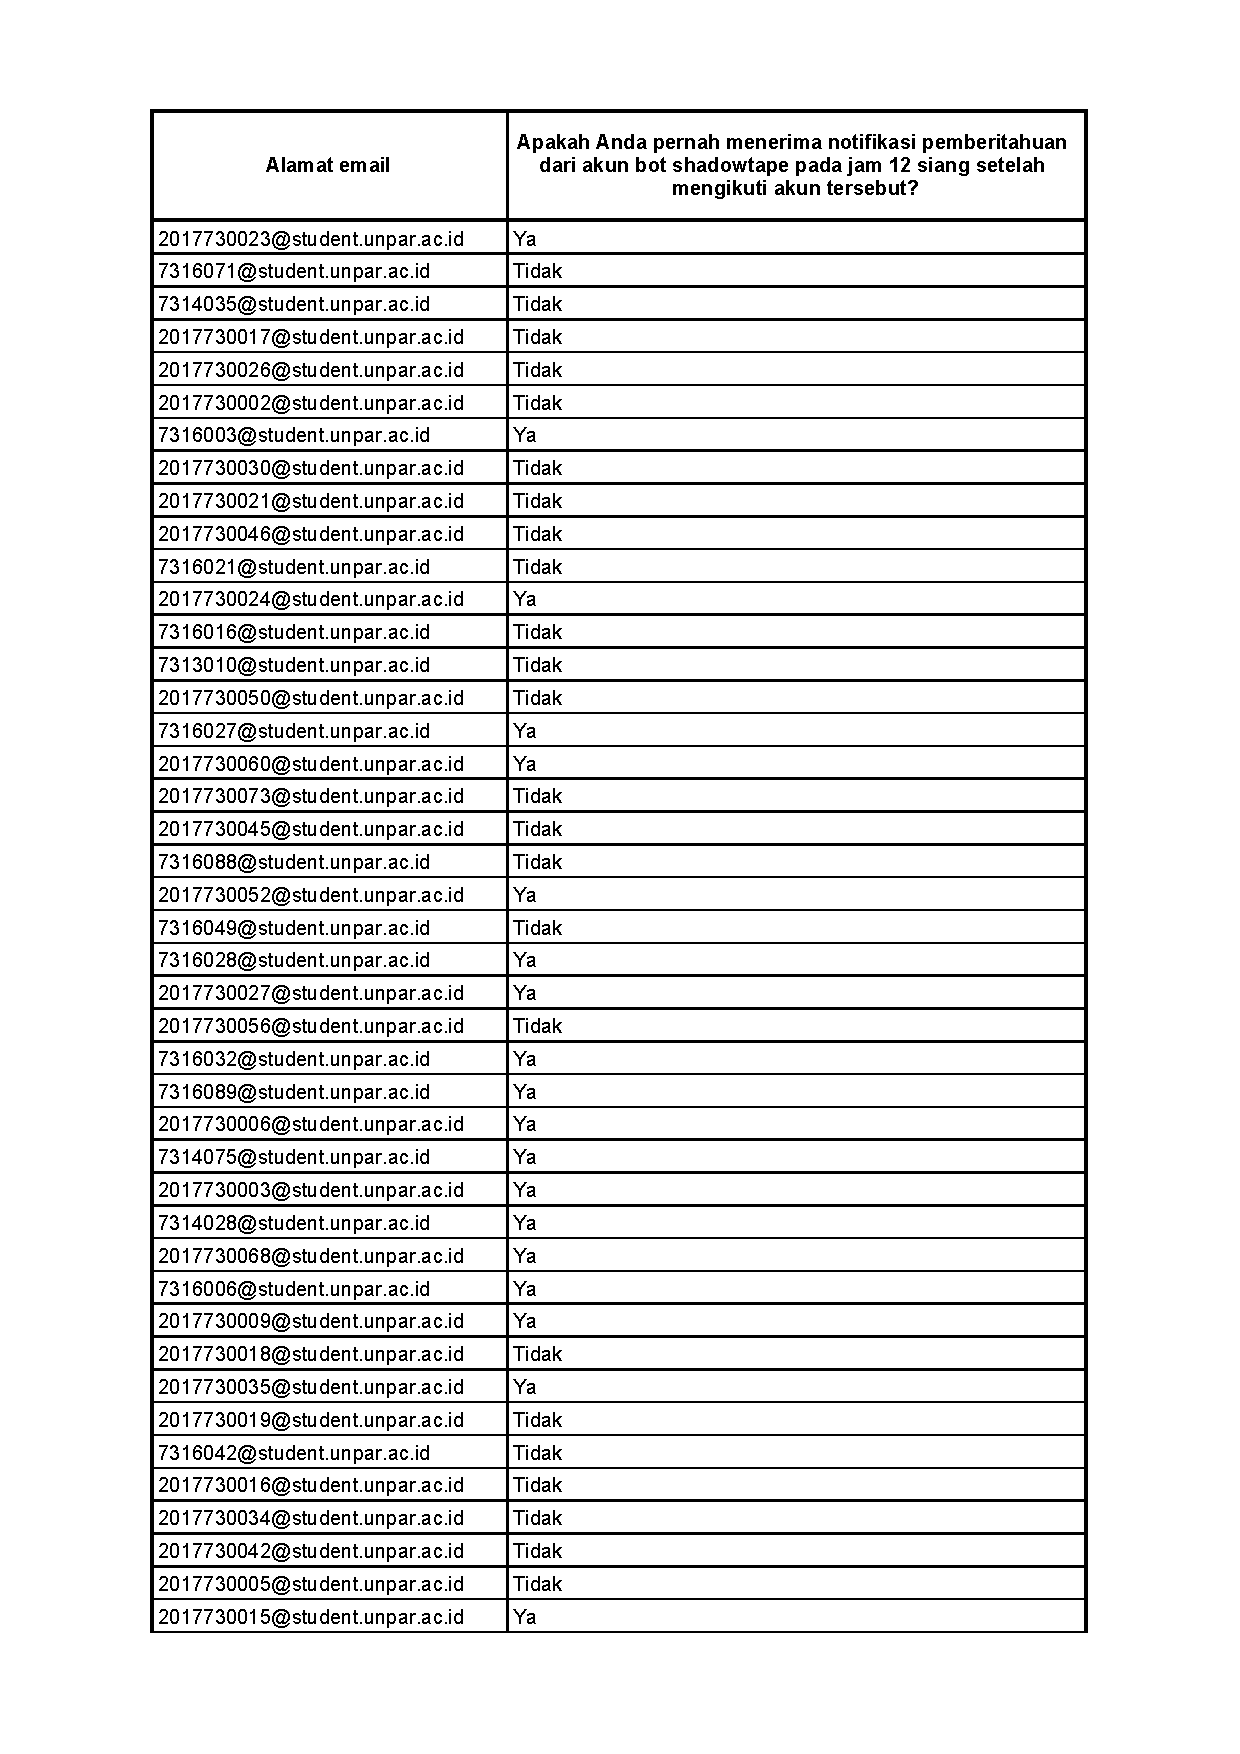
\includepdf[page=-,pagecommand={},width=\textwidth]{./Lampiran/Survey/Survey-TerimaNotifikasiLINE.pdf}
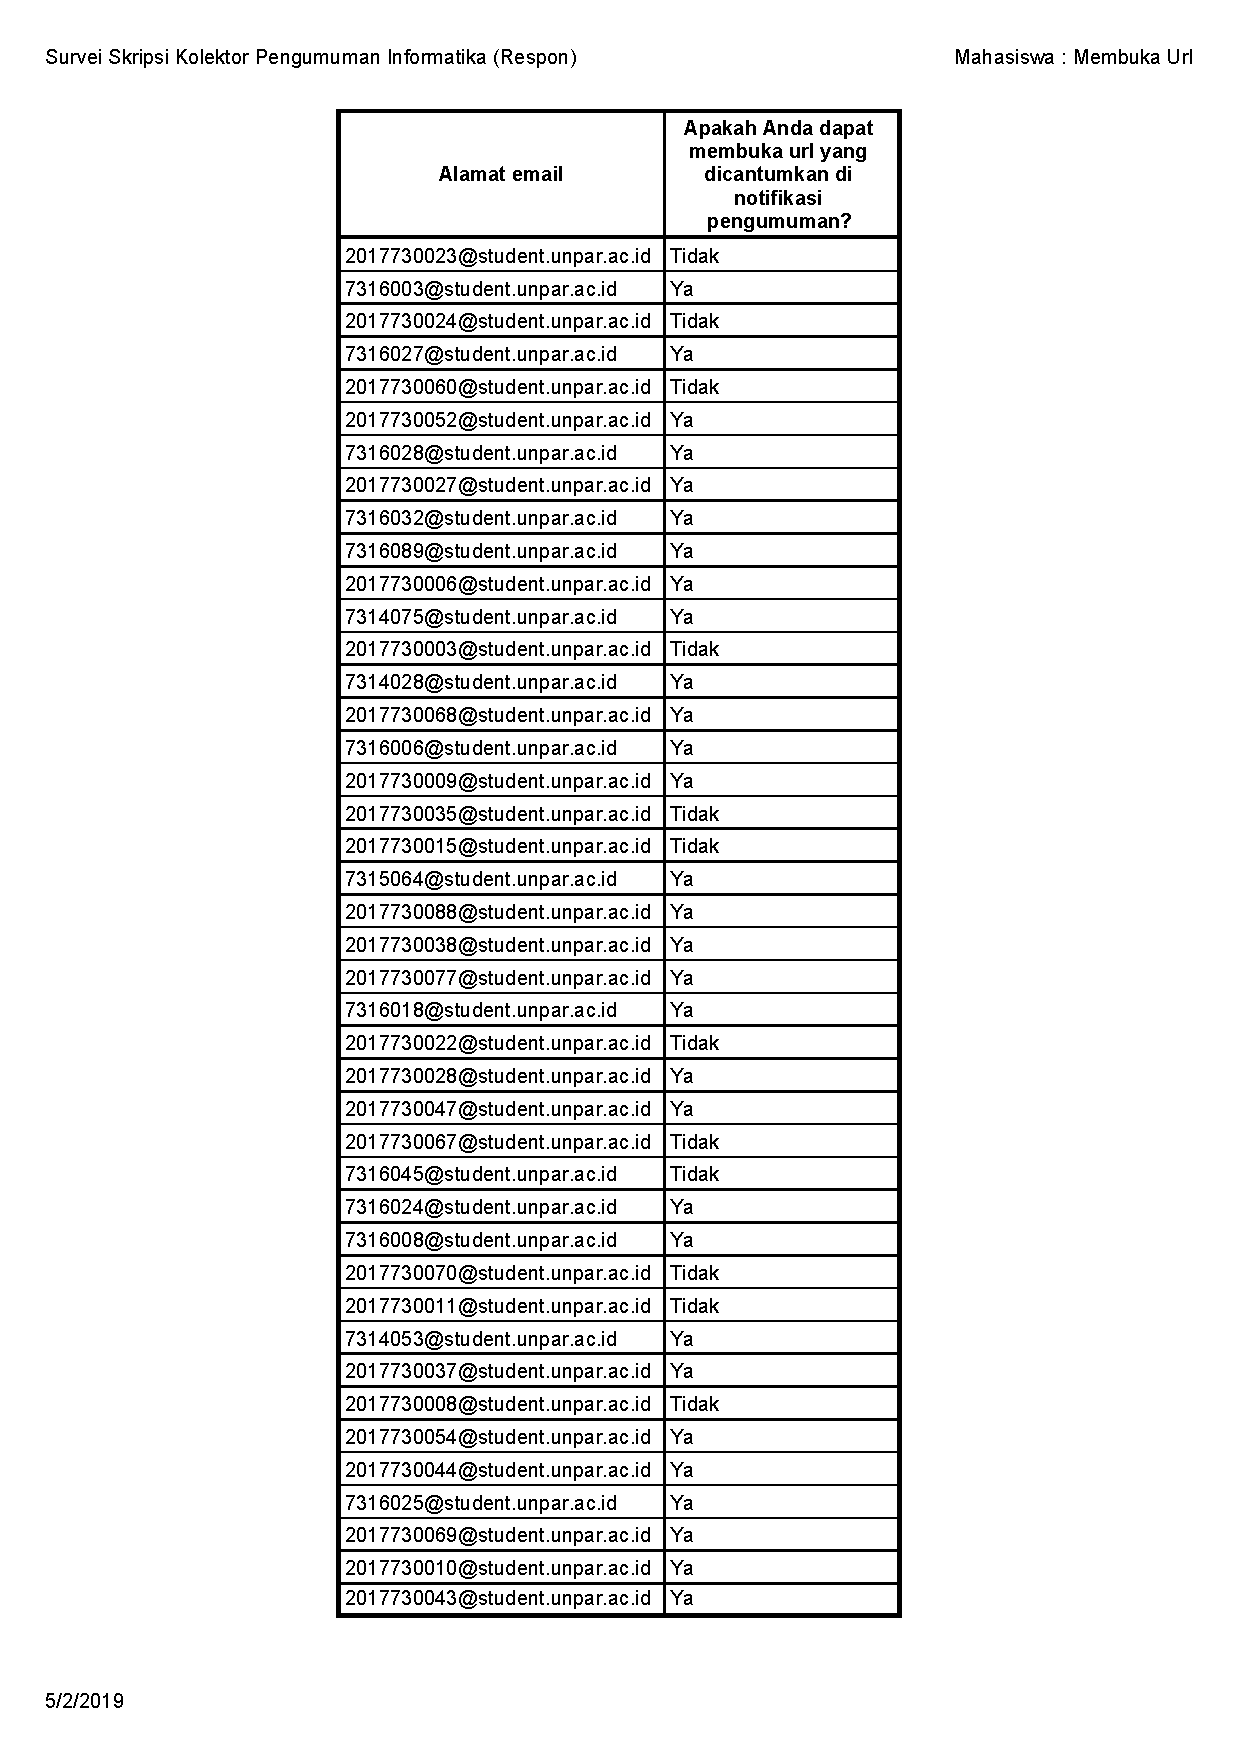
\includepdf[page=-,pagecommand={},width=\textwidth]{./Lampiran/Survey/Survey-Mahasiswa-BukaUrl.pdf}
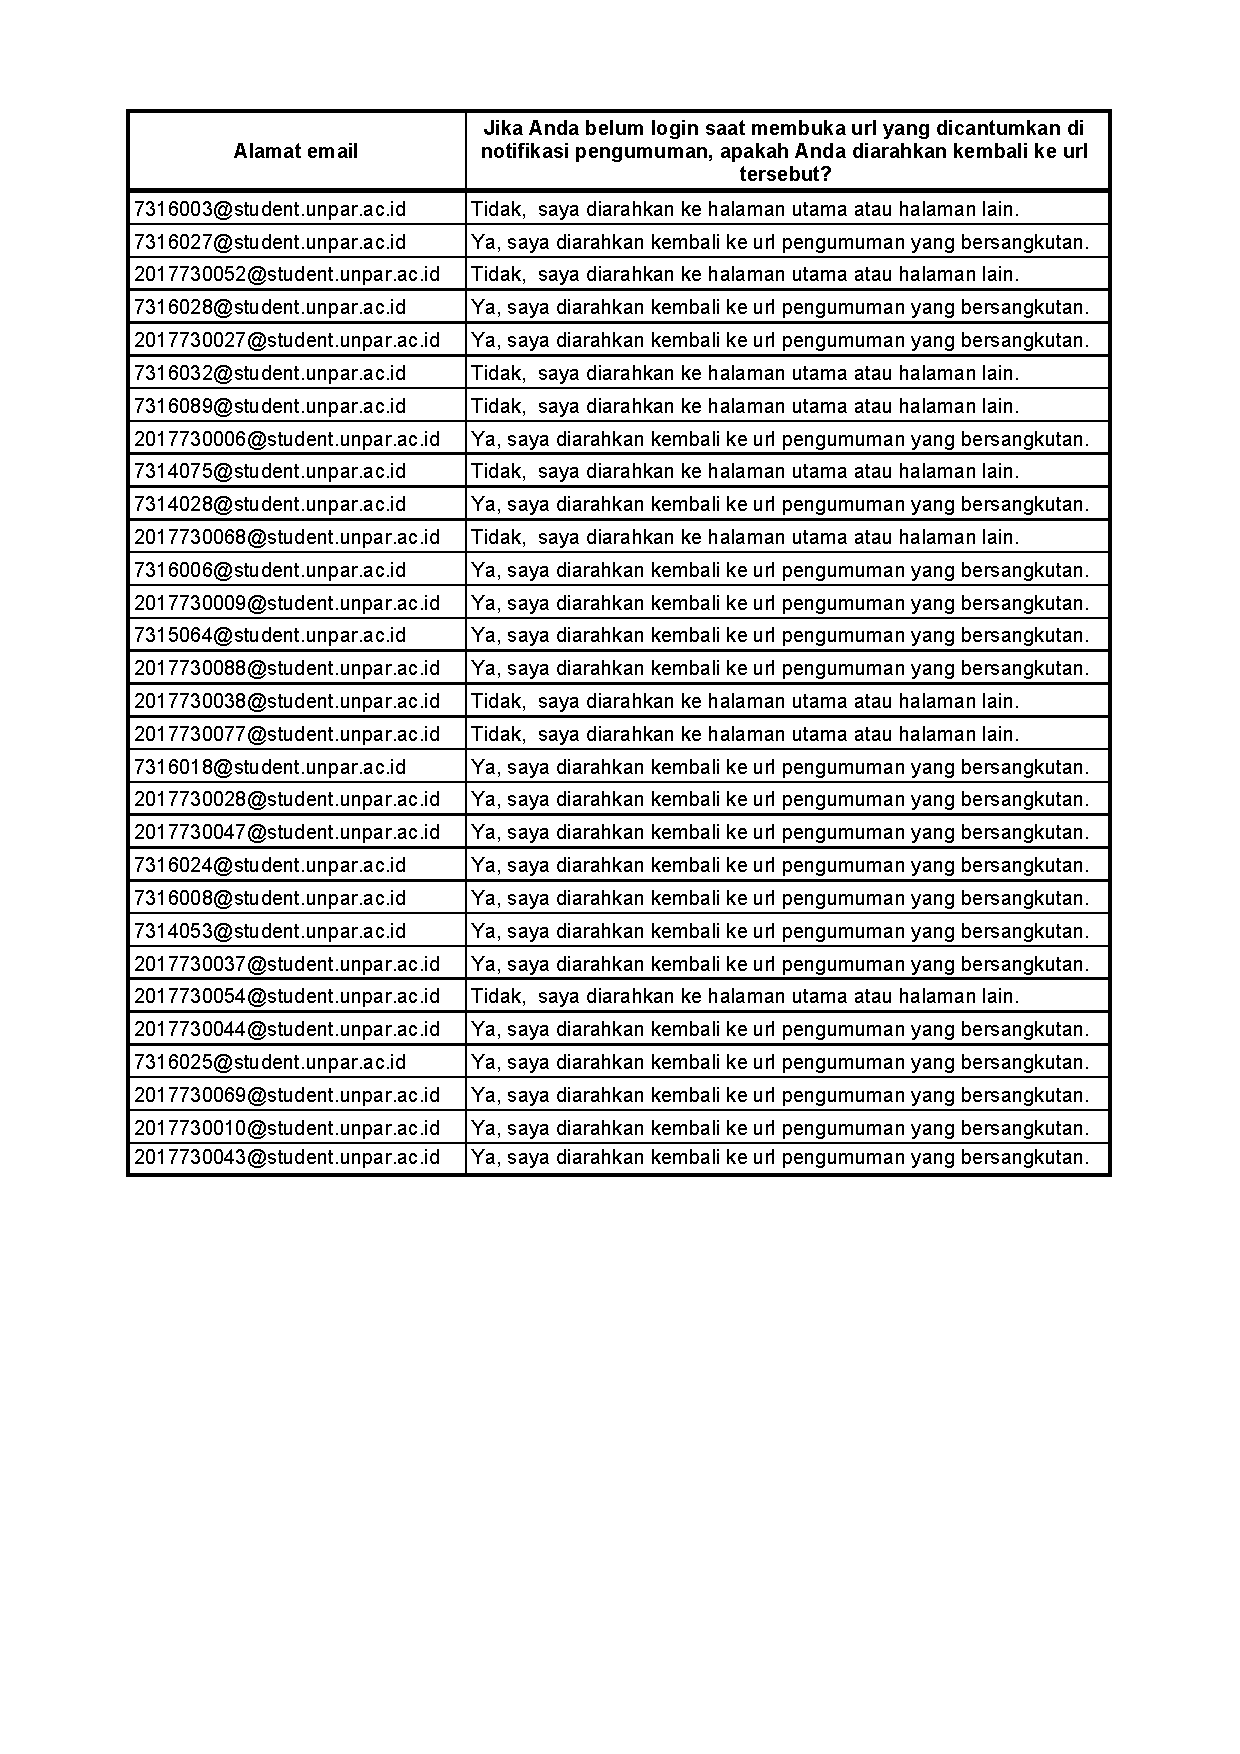
\includepdf[page=-,pagecommand={},width=\textwidth]{./Lampiran/Survey/Survey-Mahasiswa-Redirecturl.pdf}
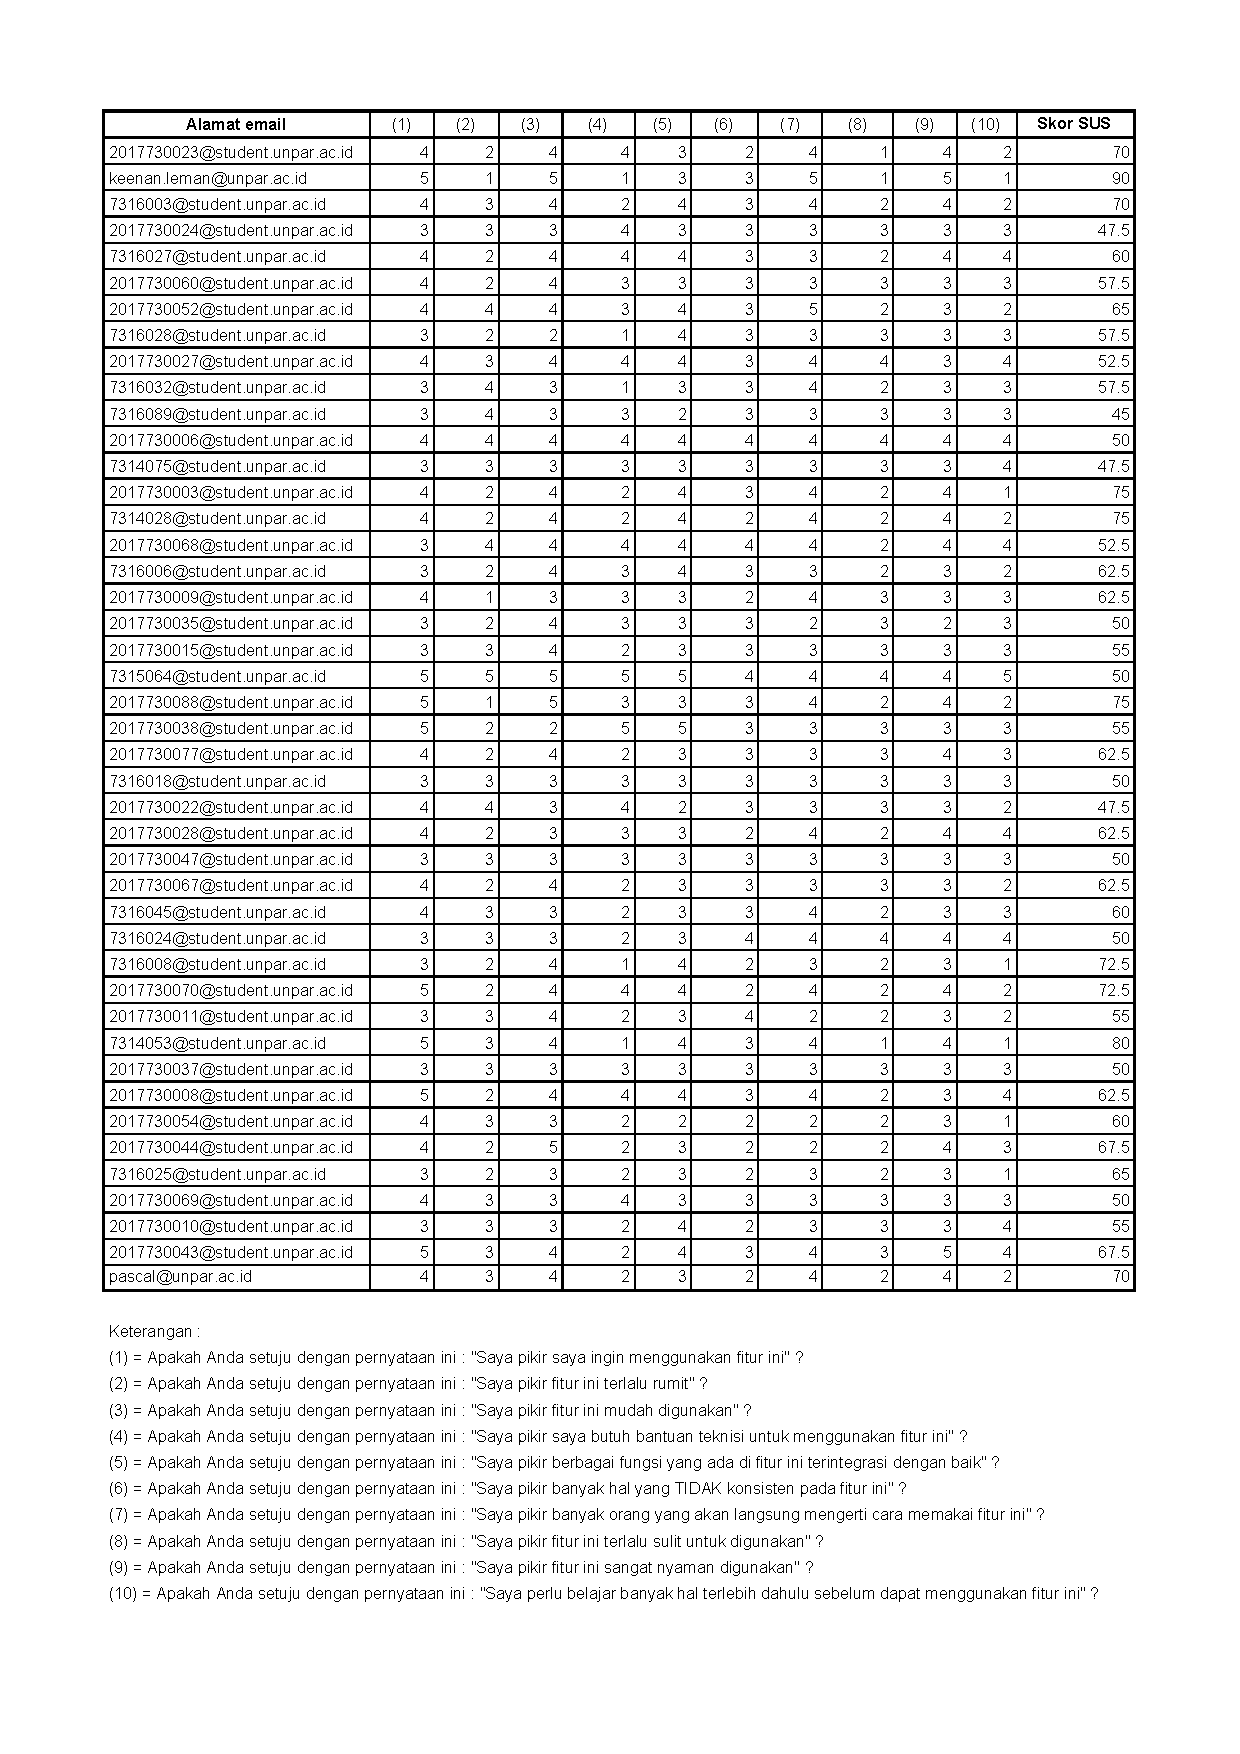
\includepdf[page=-,pagecommand={},width=\textwidth]{./Lampiran/Survey/Survey-SUS.pdf}
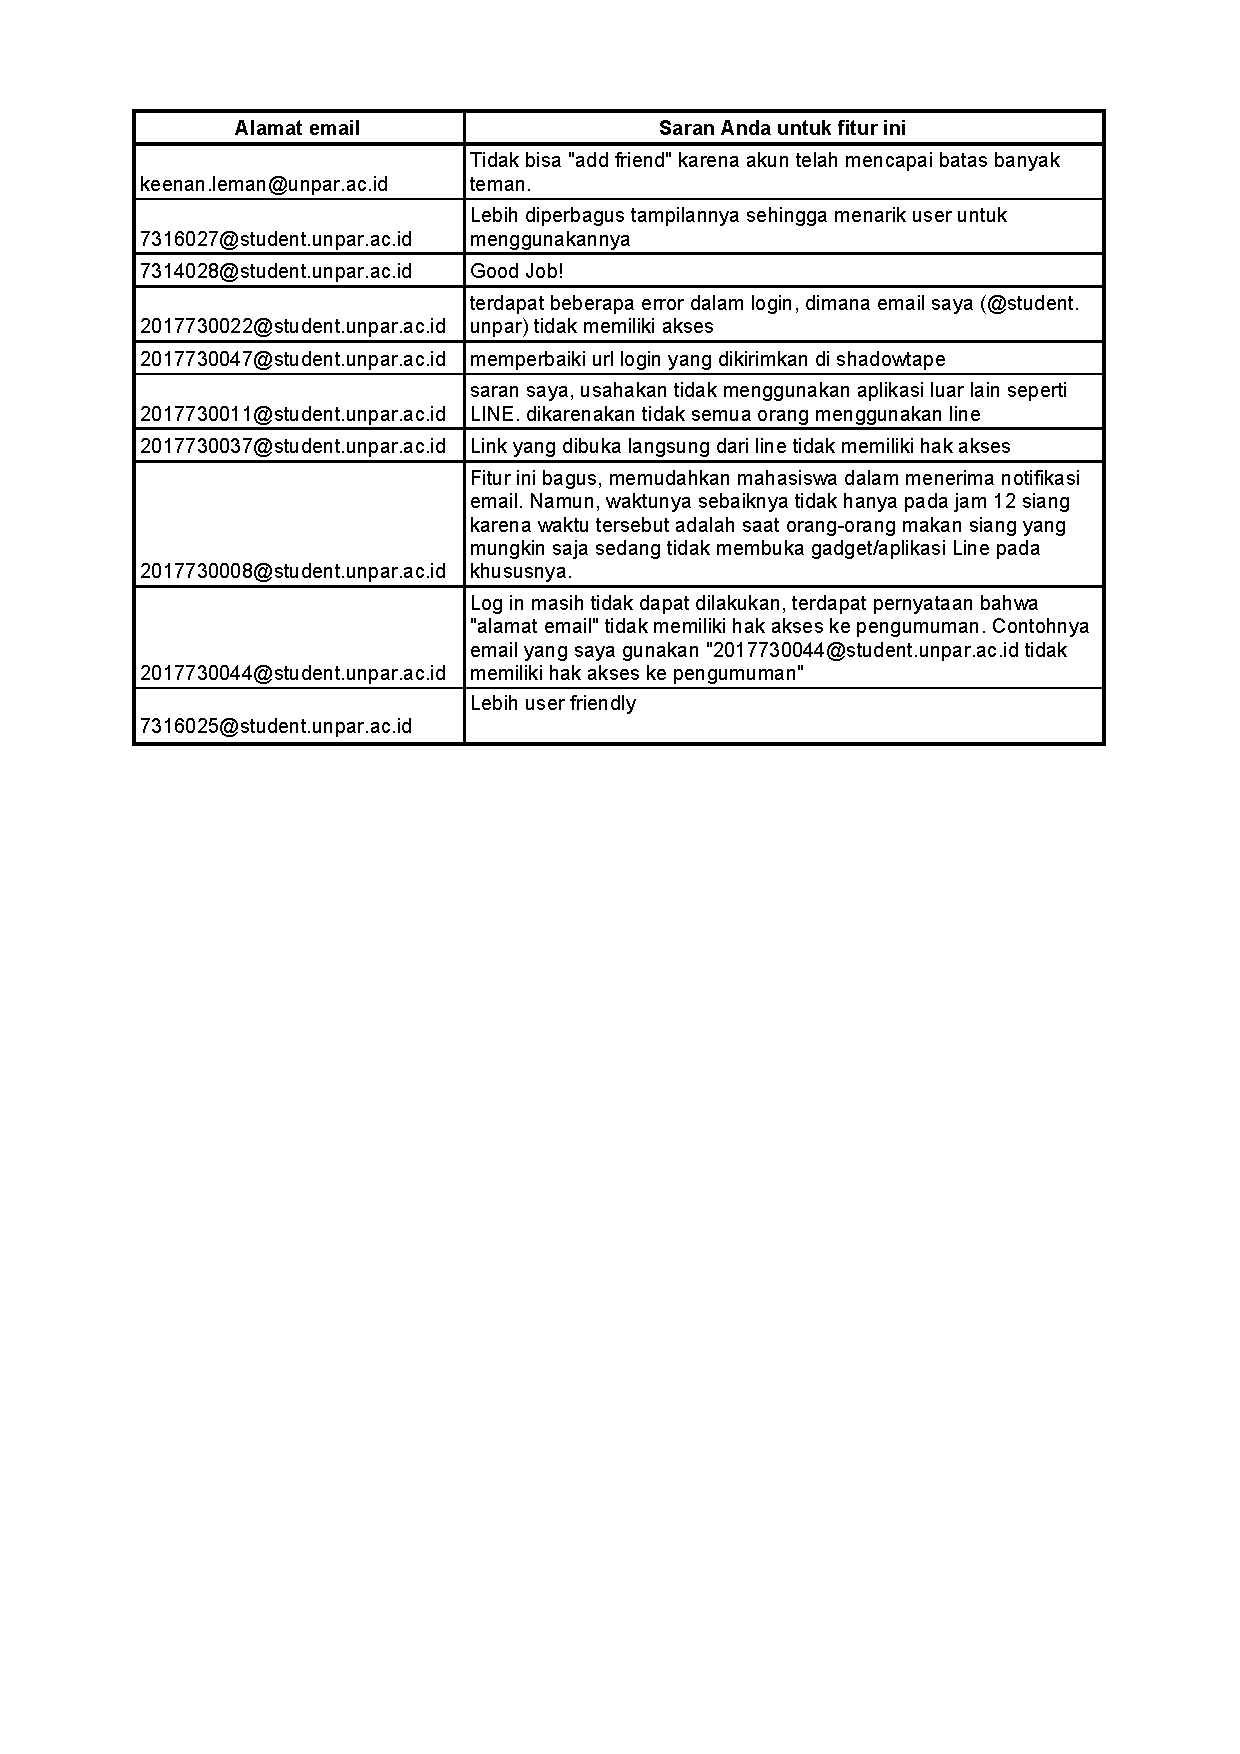
\includepdf[page=-,pagecommand={},width=\textwidth]{./Lampiran/Survey/Survey-Saran.pdf}

\section{Rangkuman Hasil Kuesioner}
\label{sec:summary-result-survey}

\begin{figure}[H]
	\centering  
	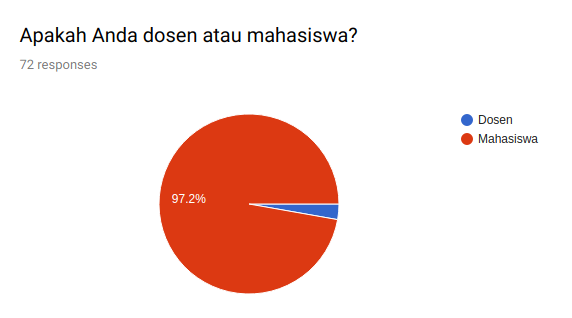
\includegraphics[scale=0.5]{./Survey-Summary/1-Dosen-Mahasiswa.png}
	\caption[Diagram profil responden]{Diagram profil responden} 
	\label{fig:summary-1-Dosen-Mahasiswa} 
\end{figure}

\begin{figure}[H]
	\centering  
	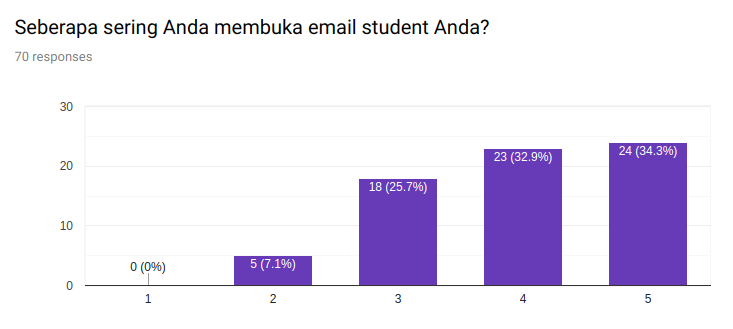
\includegraphics[scale=0.5]{./Survey-Summary/2-Penggunaan-Email.png}
	\caption[Diagram penggunaan email di kalangan mahasiswa]{Diagram penggunaan email di kalangan mahasiswa} 
	\label{fig:summary-2-Penggunaan-Email} 
\end{figure}

\begin{figure}[H]
	\centering  
	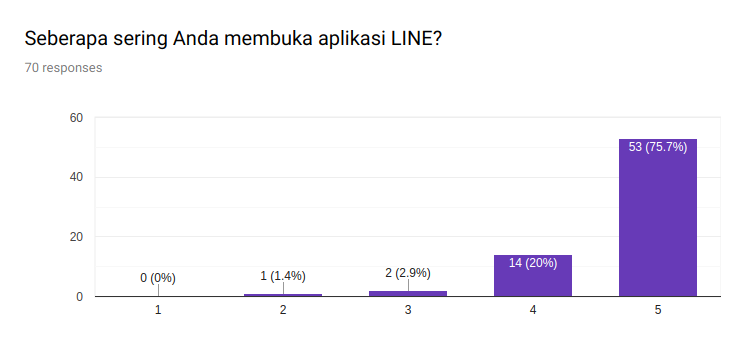
\includegraphics[scale=0.5]{./Survey-Summary/3-Penggunaan-LINE.png}
	\caption[Diagram penggunaan LINE di kalangan mahasiswa]{Diagram penggunaan LINE di kalangan mahasiswa} 
	\label{fig:summary-3-Penggunaan-LINE} 
\end{figure}

\begin{figure}[H]
	\centering  
	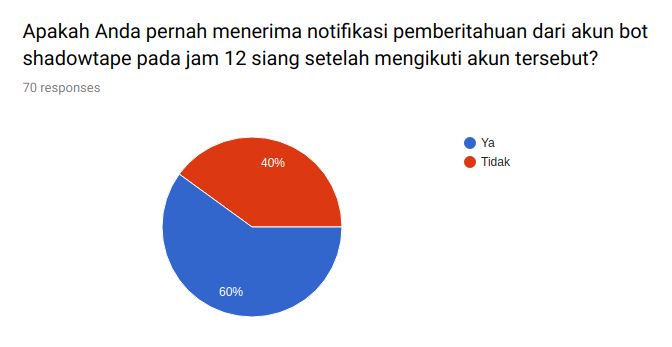
\includegraphics[scale=0.5]{./Survey-Summary/4-Notifikasi-LINE.png}
	\caption[Diagram mahasiswa yang menerima notifikasi LINE]{Diagram mahasiswa yang menerima notifikasi LINE} 
	\label{fig:summary-4-Notifikasi-LINE} 
\end{figure}

\begin{figure}[H]
	\centering  
	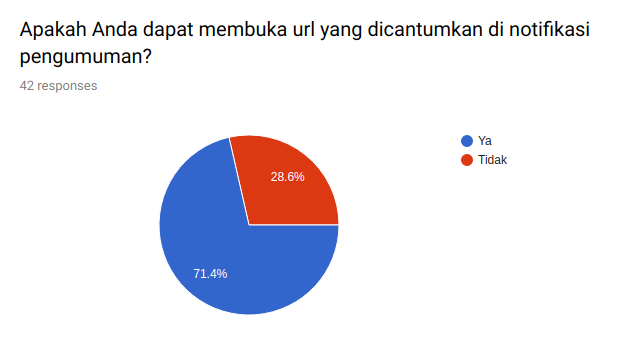
\includegraphics[scale=0.5]{./Survey-Summary/5-Buka-Url.png}
	\caption[Diagram mahasiswa yang dapat membuka url pengumuman]{Diagram mahasiswa yang dapat membuka url pengumuman} 
	\label{fig:summary-5-Buka-Url} 
\end{figure}

\begin{figure}[H]
	\centering  
	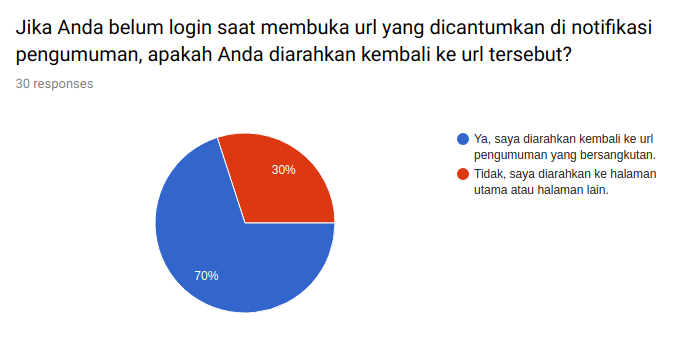
\includegraphics[scale=0.5]{./Survey-Summary/6-Redirect-url.png}
	\caption[Diagram mahasiswa yang diarahkan kembali ke url pengumuman setelah login]{Diagram mahasiswa yang diarahkan kembali ke url pengumuman setelah login} 
	\label{fig:summary-6-Redirect-url} 
\end{figure}

\begin{figure}[H]
	\centering  
	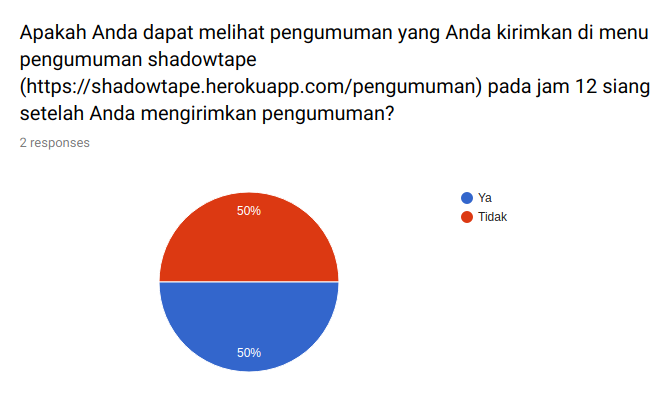
\includegraphics[scale=0.5]{./Survey-Summary/7-Dosen-Lihat-Pengumuman.png}
	\caption[Diagram dosen yang dapat melihat pengumuman yang diumumkannya]{Diagram dosen yang dapat melihat pengumuman yang diumumkannya} 
	\label{fig:summary-7-Dosen-Lihat-Pengumuman} 
\end{figure}

\begin{figure}[H]
	\centering  
	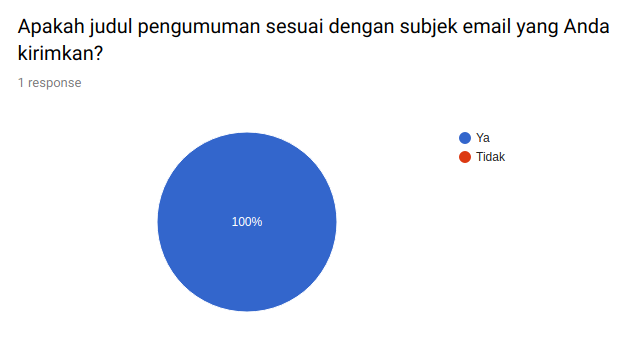
\includegraphics[scale=0.5]{./Survey-Summary/8-Dosen-Judul.png}
	\caption[Diagram dosen yang judul pengumumannya sesuai dengan subjek email yang ia kirim]{Diagram dosen yang judul pengumumannya sesuai dengan subjek email yang ia kirim} 
	\label{fig:summary-8-Dosen-Judul} 
\end{figure}

\begin{figure}[H]
	\centering  
	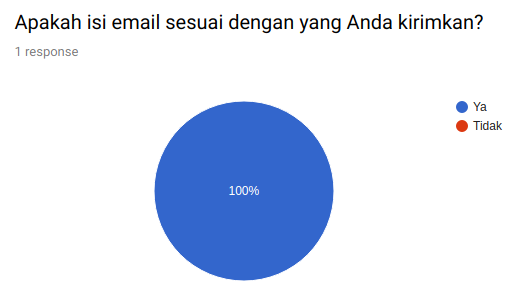
\includegraphics[scale=0.5]{./Survey-Summary/9-Dosen-Isi.png}
	\caption[Diagram dosen yang isi pengumumannya sesuai dengan isi email yang ia kirim]{Diagram dosen yang isi  pengumumannya sesuai dengan isi email yang ia kirim} 
	\label{fig:summary-9-Dosen-Isi} 
\end{figure}

\begin{figure}[H]
	\centering  
	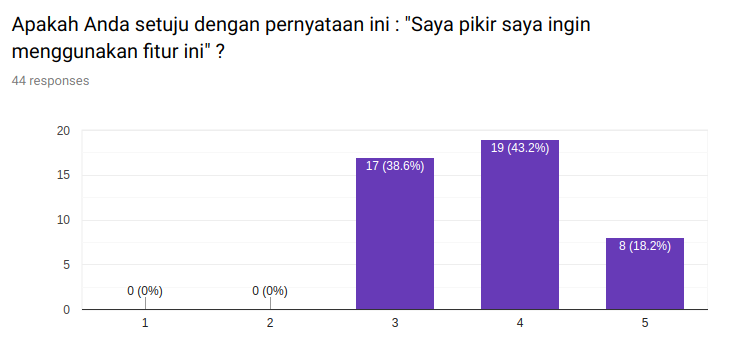
\includegraphics[scale=0.5]{./Survey-Summary/SUS-1.png}
	\caption[Diagram jawaban pertanyaan System Usability Scale yang pertama]{Diagram jawaban pertanyaan System Usability Scale yang pertama} 
	\label{fig:summary-SUS-1} 
\end{figure}

\begin{figure}[H]
	\centering  
	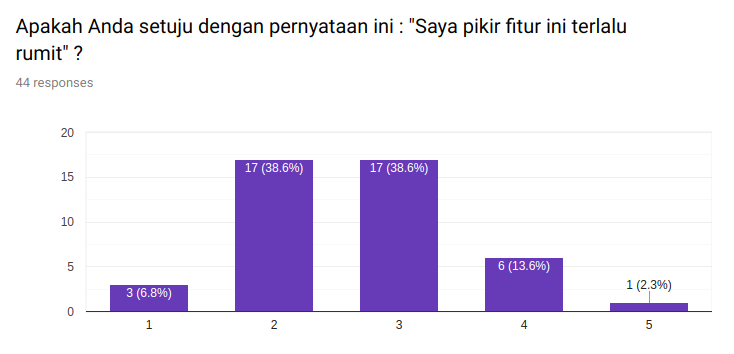
\includegraphics[scale=0.5]{./Survey-Summary/SUS-2.png}
	\caption[Diagram jawaban pertanyaan System Usability Scale yang kedua]{Diagram jawaban pertanyaan System Usability Scale yang kedua} 
	\label{fig:summary-SUS-2} 
\end{figure}

\begin{figure}[H]
	\centering  
	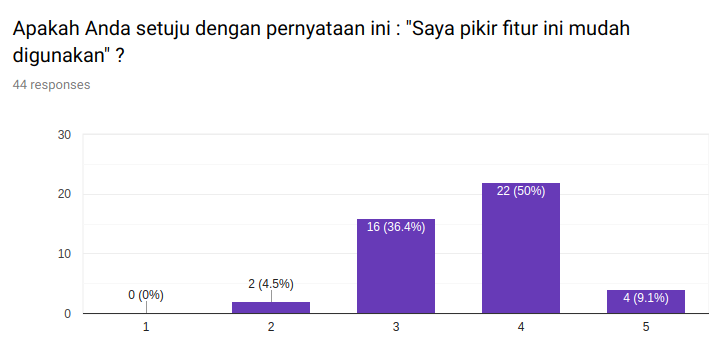
\includegraphics[scale=0.5]{./Survey-Summary/SUS-3.png}
	\caption[Diagram jawaban pertanyaan System Usability Scale yang ketiga]{Diagram jawaban pertanyaan System Usability Scale yang ketiga} 
	\label{fig:summary-SUS-3} 
\end{figure}

\begin{figure}[H]
	\centering  
	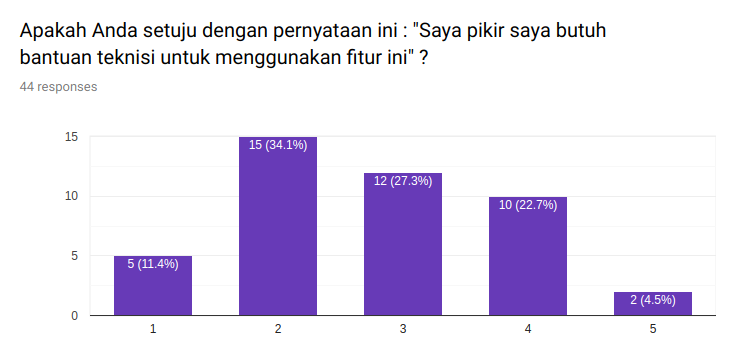
\includegraphics[scale=0.5]{./Survey-Summary/SUS-4.png}
	\caption[Diagram jawaban pertanyaan System Usability Scale yang keempat]{Diagram jawaban pertanyaan System Usability Scale yang keempat} 
	\label{fig:summary-SUS-4} 
\end{figure}

\begin{figure}[H]
	\centering  
	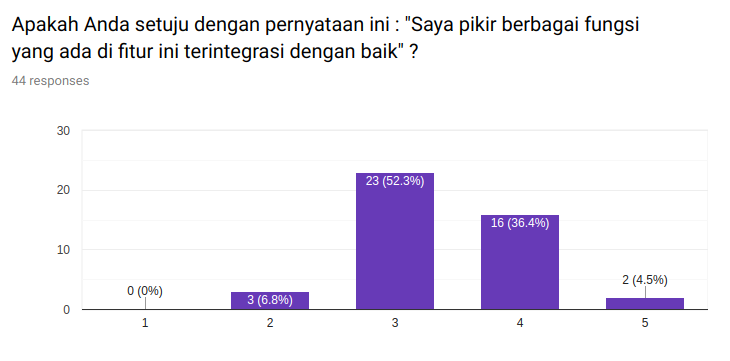
\includegraphics[scale=0.5]{./Survey-Summary/SUS-5.png}
	\caption[Diagram jawaban pertanyaan System Usability Scale yang kelima]{Diagram jawaban pertanyaan System Usability Scale yang kelima} 
	\label{fig:summary-SUS-5} 
\end{figure}

\begin{figure}[H]
	\centering  
	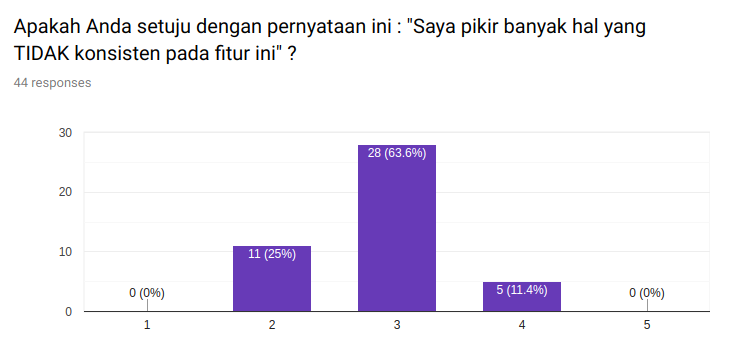
\includegraphics[scale=0.5]{./Survey-Summary/SUS-6.png}
	\caption[Diagram jawaban pertanyaan System Usability Scale yang keenam]{Diagram jawaban pertanyaan System Usability Scale yang keenam} 
	\label{fig:summary-SUS-6} 
\end{figure}

\begin{figure}[H]
	\centering  
	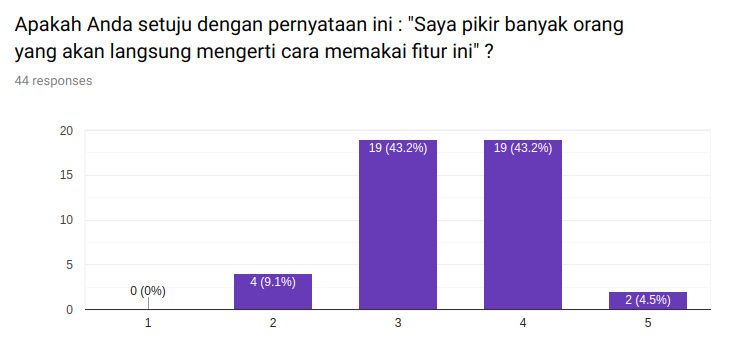
\includegraphics[scale=0.5]{./Survey-Summary/SUS-7.png}
	\caption[Diagram jawaban pertanyaan System Usability Scale yang ketujuh]{Diagram jawaban pertanyaan System Usability Scale yang ketujuh} 
	\label{fig:summary-SUS-7} 
\end{figure}

\begin{figure}[H]
	\centering  
	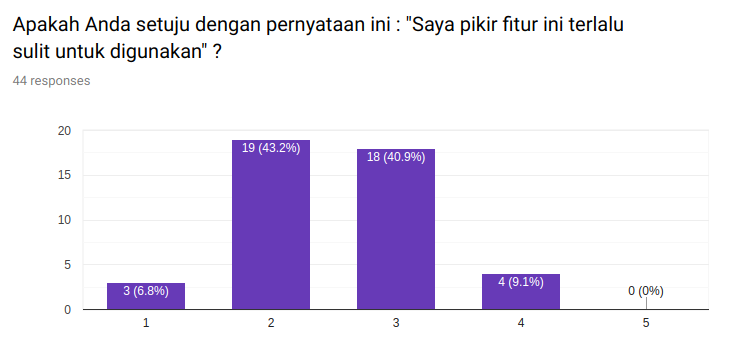
\includegraphics[scale=0.5]{./Survey-Summary/SUS-8.png}
	\caption[Diagram jawaban pertanyaan System Usability Scale yang kedelapan]{Diagram jawaban pertanyaan System Usability Scale yang kedelapan} 
	\label{fig:summary-SUS-8} 
\end{figure}

\begin{figure}[H]
	\centering  
	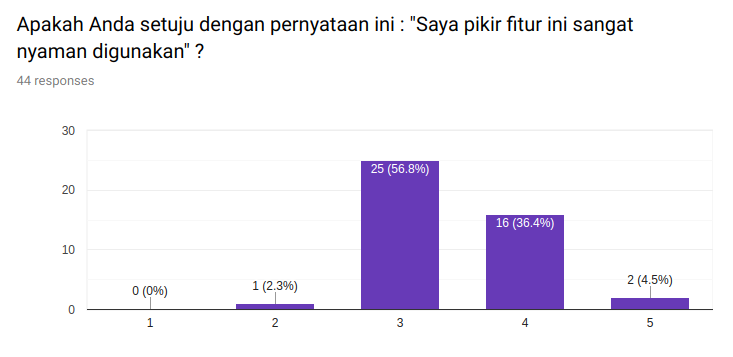
\includegraphics[scale=0.5]{./Survey-Summary/SUS-9.png}
	\caption[Diagram jawaban pertanyaan System Usability Scale yang kesembilan]{Diagram jawaban pertanyaan System Usability Scale yang kesembilan} 
	\label{fig:summary-SUS-9} 
\end{figure}

\begin{figure}[H]
	\centering  
	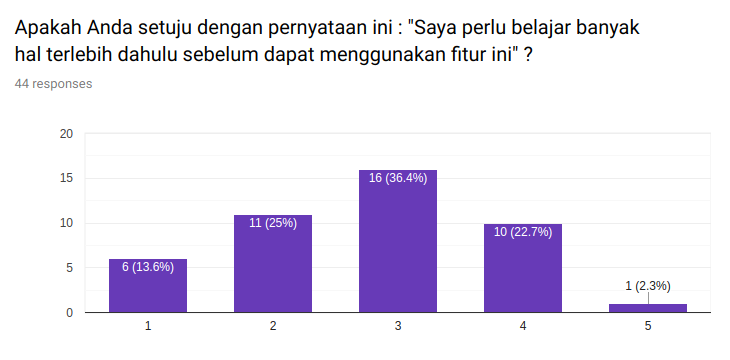
\includegraphics[scale=0.5]{./Survey-Summary/SUS-10.png}
	\caption[Diagram jawaban pertanyaan System Usability Scale yang kesepuluh]{Diagram jawaban pertanyaan System Usability Scale yang kesepuluh} 
	\label{fig:summary-SUS-10} 
\end{figure}